%% ============================================================
%%  Scalable Multi-Robot Coordination: Integrating LCBA Task
%%  Allocation with Decentralized Path Planning
%%
%%  Master of Science in Engineering Thesis
%%  University of Pennsylvania, School of Engineering and Applied Science
%%  Department of Electrical and Systems Engineering
%%
%%  Author : Shreyas [Last Name]
%%  Advisor: [Advisor Name]
%%  Date   : April 2026
%% ============================================================

\documentclass[12pt, oneside]{report}

%% ── Page geometry ───────────────────────────────────────────────
\usepackage[
  top=1in, bottom=1in,
  left=1.5in, right=1in   % wider left margin for binding
]{geometry}

%% ── Core packages ───────────────────────────────────────────────
\usepackage{amsmath, amssymb, amsthm}   % math
\usepackage{graphicx}                   % figures
\usepackage{subcaption}                 % subfigures
\usepackage{booktabs}                   % professional tables
\usepackage{multirow}                   % table cells spanning rows
\usepackage{array}                      % extended table formatting
\usepackage{algorithm}                  % algorithm floats
\usepackage{algpseudocode}              % pseudocode inside algorithms
\usepackage{xcolor}                     % colors
\usepackage{hyperref}                   % clickable links and cross-refs
\usepackage{cleveref}                   % smart cross-referencing (Cref)
\usepackage{natbib}                     % author-year or numbered citations
\usepackage{setspace}                   % line spacing
\usepackage{fancyhdr}                   % headers and footers
\usepackage{tikz}                       % diagrams (optional)
\usetikzlibrary{shapes.geometric, arrows.meta, positioning, fit}
\usepackage{pgfplots}                   % plots directly in LaTeX (optional)
\pgfplotsset{compat=1.18}
\usepackage{enumitem}                   % better list control
\usepackage[protrusion=true,expansion=true,tracking=true,kerning=true,spacing=true]{microtype} % better text justification
\usepackage{lmodern}                    % better font rendering
\usepackage[T1]{fontenc}

%% ── Hyperref setup ──────────────────────────────────────────────
\hypersetup{
  colorlinks = true,
  linkcolor  = black,
  citecolor  = blue,
  urlcolor   = blue,
  pdftitle   = {Scalable Multi-Robot Coordination: Integrating LCBA
                Task Allocation with Decentralized Path Planning},
  pdfauthor  = {Shreyas},
}

%% ── Line spacing (Penn typically requires double or 1.5) ────────
\onehalfspacing

%% ── Header / footer ─────────────────────────────────────────────
\pagestyle{fancy}
\fancyhf{}
\fancyhead[L]{\nouppercase{\leftmark}}
\fancyhead[R]{\thepage}
\renewcommand{\headrulewidth}{0.4pt}

%% ── Theorem environments ────────────────────────────────────────
\newtheorem{theorem}{Theorem}[chapter]
\newtheorem{lemma}[theorem]{Lemma}
\newtheorem{proposition}[theorem]{Proposition}
\newtheorem{corollary}[theorem]{Corollary}
\theoremstyle{definition}
\newtheorem{definition}[theorem]{Definition}
\theoremstyle{remark}
\newtheorem{remark}[theorem]{Remark}

%% ── Custom commands ─────────────────────────────────────────────
\newcommand{\Na}{N_a}           % number of agents
\newcommand{\Nt}{N_t}           % number of tasks
\newcommand{\Lt}{L_t}           % capacity per agent
\newcommand{\comm}{r_{\text{comm}}} % communication range
\newcommand{\todo}[1]{\textcolor{red}{\textbf{[TODO: #1]}}}
\newcommand{\note}[1]{\textcolor{blue}{\textit{[Note: #1]}}}

%% ── Figure path ─────────────────────────────────────────────────
\graphicspath{{figures/}}

%% ============================================================
\begin{document}

%% ── Front matter ────────────────────────────────────────────────
\pagenumbering{roman}
\pagestyle{plain}

%% ============================================================
%%  Title Page
%% ============================================================
\begin{titlepage}
  \singlespacing
  \centering
  \vspace*{0.4in}

  {\normalsize
    \MakeUppercase{Scalable Multi-Robot Coordination: Integrating LCBA Task
    Allocation with Decentralized Path Planning}
  \par}

  \vspace{0.25in}

  {\normalsize Shreyas Raorane\par}

  \vspace{0.45in}

  {\normalsize A THESIS\par}

  \vspace{0.12in}

  {\normalsize in\par}

  \vspace{0.12in}

  {\normalsize Master of Science in Engineering in Robotics\par}

  \vspace{0.3in}

  {\normalsize Presented to the Faculties of the University of Pennsylvania\par}

  \vspace{0.12in}

  {\normalsize in\par}

  \vspace{0.12in}

  {\normalsize Partial Fulfillment of the Requirements for the\par}

  \vspace{0.08in}

  {\normalsize Degree of Master of Science in Engineering\par}

  \vspace{0.08in}

  {\normalsize 2026\par}

  \vspace{0.35in}

  \begin{flushleft}
    \rule{2.5in}{0.4pt}\\[2pt]
    Linh Thi Xuan Phan\\
    Professor, Computer and Information Science, University of Pennsylvania\\
    Supervisor of Thesis
  \end{flushleft}

  \vspace{0.15in}

  \begin{flushleft}
    \rule{2.5in}{0.4pt}\\[2pt]
    Rahul Mangharam\\
    Professor, Electrical and Systems Engineering, University of Pennsylvania\\
    Supervisor of Thesis
  \end{flushleft}

  \vspace{0.15in}

  \begin{flushleft}
    \rule{2.5in}{0.4pt}\\[2pt]
    M. Ani Hsieh\\
    Associate Professor, Mechanical Engineering and Applied Mechanics, University of Pennsylvania\\
    Program Chair
  \end{flushleft}

\end{titlepage}

% ============================================================
%  Abstract
% ============================================================
\chapter*{Abstract}
\addcontentsline{toc}{chapter}{Abstract}

Decentralized multi-robot task allocation (MRTA) methods such as
CBBA~\cite{choi2009consensus} and its successor
GCBBA~\cite{kha2025enhancing} assume fully connected or at least static
communication graphs.
These assumptions rarely hold in deployments where range-limited radios,
obstacles, and robot mobility create dynamic, intermittently disconnected
topologies.
This thesis presents the \textbf{Local Consensus-Based Bundle Algorithm (LCBA)},
which extends GCBBA by replacing its global consensus requirement with
component-local consensus.
LCBA relaxes three key assumptions of its predecessors:
(1)~tasks need not be known \emph{a priori}; LCBA handles dynamic,
steady-state arrivals via event-driven replanning;
(2)~the communication graph may be arbitrarily disconnected; agents restrict
consensus to their current connected component and resolve conflicts upon
reconnection; and
(3)~the communication topology may change at every timestep.

LCBA is integrated with three interchangeable path planning strategies
(Cooperative A*, Priority-Based Search, and Rolling Horizon Collision
Resolution) forming a complete multi-robot coordination pipeline with a
modular, planner-agnostic allocation layer.
The system is evaluated across six gridworld environments of increasing scale
(30$\times$30 with 6 agents, 44$\times$28 with 12 agents, 36$\times$36 with
20 agents, 60$\times$60 with 18 agents, 72$\times$72 with 80 agents, and
161$\times$63 with 200 agents) against three baselines: CBBA, the centralized
Sequential Greedy Algorithm~(SGA), and the state-of-the-art decentralized
method DMCHBA~\cite{samiei2024dmchba}.

Experiments are conducted in two modes.
In batch mode (fixed task set, makespan objective), LCBA achieves
non-zero task completion at all six communication ranges tested, including
settings where CBBA and SGA achieve zero completion rate.
In steady-state mode (continuous task arrivals, throughput objective),
LCBA's throughput is flat across the full communication spectrum
(from fully disconnected to fully connected) while all baselines degrade
sharply below the connectivity threshold.
On connected graphs, LCBA achieves a sub-optimality ratio of
\textbf{1.0--1.3} relative to SGA, within the theoretical
50\%-optimality bound inherited from GCBBA.
The path planner comparison reveals that CA* offers the best
computation-throughput trade-off for small fleets, while RHCR is preferred
under heavy load or for larger agent counts.

The results establish LCBA as the most robust decentralized allocation
method across the full communication spectrum, with implications for
warehouse automation, disaster response, and other domains where
communication reliability cannot be guaranteed.

%% ============================================================
%%  Acknowledgements
%% ============================================================
\chapter*{Acknowledgements}
\addcontentsline{toc}{chapter}{Acknowledgements}

First and foremost, I would like to express my sincere gratitude to my 
advisors, Dr.\ Linh Thi Xuan Phan, Dr.\ Rahul Mangharam, and Dr.\ Ani Hsieh. 
Your continuous guidance, profound insights, and immense patience have been 
invaluable throughout my master's research. Thank you for pushing me to 
maintain the highest standards of academic rigor and for providing the 
support necessary to see this massive experimental evaluation through to 
completion.

I am grateful to the members of xLAB and my peers at the University of 
Pennsylvania for their helpful discussions and for fostering a stimulating 
research environment.

I want to extend a special thank you to my friends---Mitali, Ajinkya, 
Rhythm, Prakriti, Rahul, and Kabir---for not only their encouragement and 
support, but also for keeping me grounded, making sure I took breaks, and 
offering much-needed distractions whenever the simulation runs felt endless.

Finally, none of this would have been possible without the unwavering love 
and support of my parents. A special mention and thank you to my sister, 
Anuja, for always being in my corner. Your endless belief in me and your 
unconditional support are the foundation of everything I have achieved.

\tableofcontents
\listoffigures
\listoftables

%% ── Main matter ─────────────────────────────────────────────────
\cleardoublepage
\pagenumbering{arabic}
\pagestyle{fancy}

%% ============================================================
%%  Chapter 1: Introduction
%% ============================================================
\chapter{Introduction}
\label{chap:introduction}


%% ── 1.1 ─────────────────────────────────────────────────────────
\section{Motivation}
\label{sec:intro_motivation}

Modern warehouses operate at a scale that exceeds the reach of any centralized
controller.
Amazon's fulfillment centres deploy tens of thousands of drive units; Ocado's
customer fulfillment centres run more than a thousand robots on a single grid
floor.
At peak throughput, each robot receives a new task within seconds of completing
the last one, and a fleet of hundreds must navigate shared aisles without
collision, without deadlock, and without leaving any induct station backlogged.
The coordination problem is, at its core, a continuous assignment problem:
which robot should pick up which item, in what order, along which path, and
when should the decision be revised?

Two broad strategies have emerged for tackling this problem.
\emph{Centralized} approaches gather all task and robot state at a single
planner, compute a globally optimal assignment, and broadcast instructions to
the fleet.
These methods enjoy strong theoretical guarantees. The Sequential Greedy
Algorithm~\cite{minoux1978accelerated} achieves at least half the optimal
assignment value in polynomial time and their simulation-to-deployment gap
is well understood.
Their weaknesses, however, are equally well documented: a single coordinator
represents a point of failure, scaling the coordinator's computation with fleet
size is non-trivial, and the assumption of reliable broadcast communication
is rarely met in real warehouses, where range-limited radios, metal shelving,
and high robot density produce an intermittently connected network of links.

\emph{Decentralized} approaches distribute the coordination decision across
the fleet.
Each robot runs a local planning algorithm using only the information available
within its communication neighbourhood, achieving resilience to node failures
and communication outages at the cost of solution quality guarantees.
The Consensus-Based Bundle Algorithm (CBBA)~\cite{choi2009consensus} and its
global extension GCBBA~\cite{kha2025enhancing} represent the state of the art
in this family: they provably converge to within 50\% of the optimal
assignment value on any \emph{connected} communication graph.

The critical qualification of \emph{connected} is where both methods fall
short of real-world requirements.
In a warehouse with a physical communication range of 5--10 meters,
robots spread across a 30-meter floor will frequently be in communication with
only a subset of the fleet.
When the communication graph fragments, CBBA and GCBBA may converge to
conflicting assignments (multiple robots claiming the same task) or leave
isolated robots idle.
Neither method specifies a recovery protocol for reconnection events or for
tasks that arrive while components are disconnected.
The result is a performance cliff: as the communication range drops below
the warehouse diameter, allocation quality degrades sharply or fails entirely.

Beyond connectivity, real warehouse deployments impose a second class of
constraints that academic benchmarks routinely abstract away:
\emph{operational constraints} arising from physical robot limitations.
Drive units carry finite batteries; a robot that exhausts its charge
mid-aisle becomes a stationary obstacle requiring manual retrieval.
Idle robots parked in main picking aisles force every active robot to
route around them, degrading throughput even when the fleet is not at
capacity.
These constraints interact with allocation in non-trivial ways: a task that
appears attractive to a low-energy agent may be unreachable before the
agent must divert to a charger; an idle agent holding position in a busy
corridor may block the paths of several active agents simultaneously.
A coordination system evaluated only on path quality and task completion
rate --- without modelling energy or congestion from idle robots --- will
miss these failure modes entirely and may perform poorly when deployed
on real hardware.

This thesis develops the \textbf{Local Consensus-Based Bundle Algorithm
(LCBA)}, which removes the connectivity assumption from GCBBA while preserving
its convergence guarantees within each connected component and extending
its correctness to dynamic, intermittently disconnected topologies.
LCBA is integrated with a family of three collision-free path planning strategies
to form a complete multi-robot coordination pipeline that can be evaluated
across a wide range of operating conditions.

The practical scope extends beyond warehouse automation.
Underwater robotic surveys operate without GPS and with highly attenuated
acoustic communication, producing exactly the intermittent connectivity
structure that LCBA is designed to handle.
Disaster-response scenarios where physical infrastructure is damaged and
communication links are unreliable require decentralized coordination
methods that continue to function even when large portions of the team are
out of contact.
Space-based robotic systems face communication delays and blackout periods
that similarly preclude any centralized coordinator.
While this thesis focuses on the warehouse setting (which provides a reliable
set of measurable metrics and a reproducible simulation environment), the
algorithm is designed with these broader application domains in mind.


%% ── 1.2 ─────────────────────────────────────────────────────────
\section{Problem Statement}
\label{sec:intro_problem}

This thesis addresses two coupled sub-problems in a $30 \times 30$ gridworld
warehouse environment populated by $\Na = 6$ mobile agents,
$|\mathcal{S}^{\text{in}}| = 8$ induct stations, and
$|\mathcal{S}^{\text{ej}}| = 38$ eject stations.

\textbf{Sub-problem 1: Decentralized multi-robot task allocation under dynamic,
intermittently disconnected communication graphs.}
Tasks arrive continuously at induct stations over time, not as a fixed batch at
$t = 0$.
Agents communicate over a proximity-based wireless channel whose topology
changes every timestep as agents move.
The communication graph may be arbitrarily disconnected: in the worst case,
each agent forms its own isolated component.
The allocation method must correctly assign tasks, resolve conflicts, and
reassign work as the topology changes. More importantly, it must operate
using only information locally
available within each agent's communication neighbourhood.
Existing methods (CBBA, GCBBA, DMCHBA) break down or stall when the graph is
persistently disconnected.

\textbf{Sub-problem 2: Collision-free execution of allocated tasks.}
Once tasks are assigned, agents must navigate from their current positions to
the assigned induct station, pick up the item, and deliver it to the assigned
eject station, all without occupying the same grid cell as another agent at the
same timestep.
The path planning method must be computationally feasible within a per-timestep
budget and must remain functional as the number of agents or the conflict
density increases.

The two sub-problems are coupled: travel-time estimates used in the allocation
algorithm depend on the paths that agents will follow, which in turn depend on
the decisions of other agents.
A practical system must handle this coupling through event-driven replanning
rather than by solving the joint problem exactly.


%% ── 1.3 ─────────────────────────────────────────────────────────
\section{Research Questions}
\label{sec:intro_questions}

The thesis investigates three research questions:

\begin{description}
  \item[\textbf{RQ1.}] Can LCBA maintain task throughput under communication
    conditions where static allocation fails?
    Specifically, does event-driven replanning allow LCBA to complete tasks
    even when the communication graph is persistently disconnected, and by how
    much does it outperform CBBA, SGA, and DMCHBA at low communication ranges?

  \item[\textbf{RQ2.}] How close to optimal (SGA) does LCBA perform as
    communication connectivity varies?
    On connected graphs where SGA is a valid reference, what is the
    sub-optimality ratio of LCBA, and does it remain within the theoretical
    50\%-optimality bound?

  \item[\textbf{RQ3.}] How do alternative path planning strategies affect
    system throughput, task wait time, and computational overhead?
    Is there a single planner that dominates across all operating conditions,
    or does the optimal choice depend on task load and agent count?
\end{description}


%% ── 1.4 ─────────────────────────────────────────────────────────
\section{Contributions}
\label{sec:intro_contributions}

This thesis makes the following contributions:

\begin{enumerate}
  \item \textbf{The Local Consensus-Based Bundle Algorithm (LCBA).}
        LCBA extends GCBBA to handle three challenges that GCBBA and CBBA
        cannot:
        (a) dynamic, online task arrivals via event-driven replanning;
        (b) arbitrarily disconnected communication graphs by restricting
            consensus to each connected component and resolving conflicts
            upon reconnection; and
        (c) dynamically changing communication topology by reconstructing
            the graph at every timestep.
        On connected components, LCBA inherits GCBBA's convergence to the SGA
        solution and the associated 50\%-optimality guarantee.

  \item \textbf{A hybrid, modular coordination pipeline.}
        LCBA is integrated with three interchangeable path planning strategies
        (Cooperative A*, Priority-Based Search, and Rolling Horizon Collision
        Resolution) within a single orchestration framework.
        The modular design allows the allocation and path planning components
        to be studied independently.

  \item \textbf{A dual-mode warehouse simulation.}
        The simulation supports both a \emph{batch mode} (fixed task set,
        makespan objective) for comparison with prior work, and a
        \emph{steady-state mode} (continuous task arrivals, throughput
        objective under fixed simulation and compute budgets) that better
        reflects the infinite-horizon operation of real warehouse systems.
        Both modes share the same environment, agents, and infrastructure,
        enabling direct comparison.

  \item \textbf{Empirical evaluation across 432+ experimental runs.}
        The system is evaluated across a full factorial sweep of communication
        range (6 values from fully isolated to fully connected),
        task arrival rate (12 values from light load to extreme saturation),
        path planner (3 variants), and allocation method (LCBA, CBBA, SGA, DMCHBA),
        across six environments ranging from 6 to 200 agents.
        This scale of evaluation provides statistical confidence in the results
        and reveals the interaction effects between communication conditions
        and planning strategy.

  \item \textbf{Operationally realistic simulation with charging, wait stations,
        and role-separated planners.}
        The simulation incorporates finite agent energy with proactive charging
        (agents navigate to charging stations before running out of power, with an
        energy-budget filter that prevents bids on unaffordable tasks),
        designated wait stations where idle agents park to avoid obstructing active
        corridors, and independently configurable path planners for task-executing,
        charging, and idle-parking agent roles.
        Together these features bridge the gap between typical academic MAPF benchmarks
        and the operational constraints of real warehouse deployments, ensuring that
        LCBA is evaluated under realistic pressure and that its design choices are
        exercised by the conditions they were designed to handle.
\end{enumerate}


%% ── 1.5 ─────────────────────────────────────────────────────────
\section{Thesis Outline}
\label{sec:intro_outline}

The remainder of this thesis is organized as follows.
\Cref{chap:background} reviews related work in multi-robot task allocation,
multi-agent path finding, communication-constrained coordination, and warehouse
automation, and identifies the specific gap this thesis fills.
\Cref{chap:methodology} describes the system architecture, the LCBA algorithm
and its warehouse adaptation, the three path planning strategies, the dynamic
replanning mechanism, and the baseline methods.
\Cref{chap:experiments} presents the experimental setup (including the dual
batch/steady-state design), defines all metrics, and reports quantitative
results across the full parameter sweep.
\Cref{chap:conclusion} summarizes the findings, revisits the contributions
in light of the experimental evidence, discusses limitations, and outlines
directions for future work.
%% ============================================================
%%  Chapter 2: Background and Related Work
%% ============================================================
\chapter{Background and Related Work}
\label{chap:background}

This chapter reviews the literature relevant to the two core problems addressed
in this thesis: multi-robot task allocation (Section~\ref{sec:bg_mrta}) and
multi-agent path finding (Section~\ref{sec:bg_mapf}).
Section~\ref{sec:bg_integrated} covers work that attempts to integrate the two,
Section~\ref{sec:bg_communication} reviews coordination under communication
constraints, and Section~\ref{sec:bg_warehouse} situates the work in the
context of warehouse automation.
Section~\ref{sec:bg_positioning} identifies the specific gap that this thesis
fills.


%% ── 2.1 ─────────────────────────────────────────────────────────
\section{Multi-Robot Task Allocation}
\label{sec:bg_mrta}

Multi-robot task allocation (MRTA) is the problem of deciding which robot
performs which task, and in what order, so as to optimize a system-level
objective such as makespan, total distance, or throughput.
The canonical taxonomy of \citet{gerkey2004formal} classifies MRTA problems
along three axes: \emph{single-task} (ST) versus \emph{multi-task} (MT) robots,
\emph{single-robot} (SR) versus \emph{multi-robot} (MR) tasks, and
\emph{instantaneous assignment} (IA) versus \emph{time-extended assignment}
(TA).
The warehouse problem studied in this thesis is an ST-SR-TA instance: each
robot handles one task at a time, each task requires exactly one robot, but
assignments evolve over time as new tasks arrive.

In its most general form, MRTA is NP-hard, even for single-task
robots~\cite{gerkey2004formal}.
Practical systems therefore rely either on polynomial-time approximation
algorithms with bounded sub-optimality, or on heuristic methods that sacrifice
formal guarantees for scalability.
The choice between centralized and decentralized architectures
      (Sections~\ref{subsec:bg_centralized} and~\ref{subsec:bg_decentralized})
is the primary design tension.


%% ── 2.1.1 ──────────────────────────────────────────────────────
\subsection{Centralized Approaches}
      \label{subsec:bg_centralized}

Centralized MRTA methods aggregate all information at a single planner that
computes assignments for all the agents.
The classical assignment problem (minimize total cost for a one-to-one
agent-task matching) can be solved optimally in $O(n^3)$ time by the Hungarian
algorithm~\cite{kuhn1955hungarian}.
When tasks can be assigned in any order and multiple tasks may be assigned to
each agent, integer linear programming (ILP) formulations achieve global
optimality but at exponential worst-case cost, rendering them impractical
for large fleets or compute-budgeted settings.

A widely used polynomial-time alternative is the \emph{Sequential Greedy
Algorithm} (SGA)~\cite{minoux1978accelerated}: at each step, the algorithm
selects the (agent, task) pair that offers the greatest marginal gain, assigns
the task, and repeats until no more beneficial assignments remain.
Under utility functions that satisfy the \emph{Diminishing Marginal Gain}
(DMG) property~\cite{fisher1978analysis}, SGA achieves at least half the
optimal assignment value.
This guarantee is tight: there exist instances where SGA achieves exactly
50\% of the optimum.

Centralized methods share two practical weaknesses.
First, they assume that all task and agent information is available at a single
point, which requires either a reliable broadcast channel or a dedicated
coordinator robot.
Both assumptions are fragile in the field: communication failures can prevent
the coordinator from learning about new tasks or updated agent states.
Second, single-point-of-failure: if the coordinator fails, the entire system
halts.
These limitations motivate the decentralized alternatives described next.


%% ── 2.1.2 ──────────────────────────────────────────────────────
\subsection{Decentralized Auction-Based Approaches}
      \label{subsec:bg_decentralized}

Auction-based methods distribute the allocation decision by having agents bid
on tasks and resolve conflicts through a shared consensus protocol.
\citet{gerkey2002sold} and \citet{dias2006market} provide early surveys of
market-based multi-robot coordination, establishing the framework in which
agents bid monetary values on tasks and the highest bidder is awarded the task.
While intuitive, early market-based approaches offered few formal guarantees
on solution quality.

The \emph{Consensus-Based Bundle Algorithm} (CBBA)~\cite{choi2009consensus}
introduced a principled framework that combines greedy bundle building with
a pairwise conflict resolution protocol.
Each agent independently builds a bundle of tasks it would like to execute,
computing bids based on the marginal gain of adding each task to its current
plan.
When agents communicate, they exchange bid and winner vectors and apply a set
of update/reset/leave rules to resolve conflicts.
\citeauthor{choi2009consensus} prove that CBBA converges to a valid
conflict-free assignment (no task assigned to more than one agent) on any
connected graph, and that the assignment achieves at least
50\%-optimality under DMG utilities.

CBBA's key limitation is its \emph{local} consensus protocol: each agent
communicates only with its immediate neighbors, and a single round of exchange
is performed per iteration.
On a graph of diameter $D > 1$, information originating at one node takes $D$
rounds to reach all other nodes.
If agents act on stale information before consensus is reached, conflicting
assignments can persist, and CBBA may converge to an assignment that is not
equivalent to the SGA solution~\cite{kha2025enhancing}.

The \emph{Global Consensus-Based Bundle Algorithm}
(GCBBA)~\cite{kha2025enhancing} corrects this deficiency by performing $2D$
consensus rounds per iteration, where $D$ is the communication graph diameter.
GCBBA also introduces the \emph{Repeated Path Times} (RPT) utility function,
which is provably DMG and better aligned with makespan minimization than the
simple travel-time utility used in CBBA.
Together, these changes allow GCBBA to provably converge to the SGA solution
on any connected graph and with any DMG utility function, while retaining the
decentralized character of CBBA.

GCBBA remains the starting point for this thesis; its handling of disconnected
graphs and dynamic task arrivals is the extension that LCBA provides.


%% ── 2.1.3 ──────────────────────────────────────────────────────
\subsection{Other Decentralized Methods}
      \label{subsec:bg_other_decentralized}

Beyond auction-based methods, several other decentralized approaches have been
proposed for MRTA.
\emph{Distributed Constraint Optimization Problems} (DCOPs) formulate task
allocation as a distributed optimization over coupled agent variables;
algorithms such as Max-Sum and DPOP achieve variable quality-runtime trade-offs
but do not scale well to large numbers of tasks~\cite{chakraa2023optimization}.
\emph{Market-based methods}~\cite{quinton2023mrta} use explicit price dynamics
to drive convergence, offering flexibility at the cost of unpredictable
convergence time.
\emph{Behavior-based methods}~\cite{parker1998alliance} allocate tasks
through emergent competition and reinforcement, with robustness to failures
but without assignment quality guarantees.

The most relevant recent competitor is the \emph{Distributed Matching by Clone
Hungarian-Based Algorithm} (DMCHBA)~\cite{samiei2024dmchba}, which extends
distributed Hungarian matching to multi-robot settings.
DMCHBA achieves strong empirical performance and provides theoretical
guarantees on connected graphs, making it a natural state-of-the-art
baseline for this thesis.
Like CBBA and GCBBA, DMCHBA assumes graph connectivity during each allocation
call.

The common thread across all existing decentralized methods is the assumption
of a \emph{connected} communication graph, at least at the time of allocation.
None of the methods reviewed explicitly handle the case where the graph is
persistently or intermittently disconnected across multiple replanning events.
This gap motivates the LCBA design.


%% ── 2.2 ─────────────────────────────────────────────────────────
\section{Multi-Agent Path Finding}
\label{sec:bg_mapf}

Multi-agent path finding (MAPF) is the problem of computing collision-free
paths for a team of agents from their respective start positions to their goal
positions on a shared graph~\cite{stern2019mapf}.
Formally, a \emph{vertex conflict} occurs when two agents occupy the same node
at the same timestep; an \emph{edge conflict} (or swap conflict) occurs when
two agents traverse the same edge in opposite directions within the same
timestep.
A solution is \emph{valid} if it contains no conflicts.

MAPF is NP-hard to solve optimally~\cite{stern2019mapf}, even for the simplest
cost function (sum of individual path lengths).
Practical approaches therefore trade off optimality against runtime, and the
appropriate trade-off depends heavily on the application: an offline warehouse
layout tool can afford hours of computation for an optimal solution, while an
online robot coordination system must plan within milliseconds per timestep.


%% ── 2.2.1 ──────────────────────────────────────────────────────
\subsection{Classical MAPF Solvers}
\label{subsec:bg_mapf_classical}

\emph{Conflict-Based Search} (CBS)~\cite{sharon2015conflict} is the
most influential optimal MAPF solver.
CBS operates at two levels: a high-level constraint tree (CT) that branches
on conflicts, and a low-level A* that plans each agent's path subject to
accumulated constraints.
CBS is complete and optimal with respect to sum-of-costs and has excellent
average-case performance, though its worst-case complexity is exponential in
the number of conflicts.
CBS remains the algorithm of choice when optimal solutions are needed and
agent counts are small ($n \lesssim 20$ in warehouse grids).

\emph{Windowed Hierarchical Cooperative A*}
(WHCA*)~\cite{silver2005cooperative} is an early suboptimal MAPF method that
applies cooperative A* within a fixed-size time window.
By planning only $w$ timesteps ahead, WHCA* avoids the long-horizon complexity
of full MAPF at the cost of potentially suboptimal paths near the window
boundary.
This idea is formalized and extended by the rolling horizon approach described
in Section~\ref{subsec:bg_mapf_lifelong}.

All A*-based planners share the same admissible heuristic: the shortest
single-agent path from the current cell to the goal, ignoring other
agents~\cite{hart1968astar}.
This heuristic is consistent, ensuring that A* explores nodes in non-decreasing
order of $f$-value and does not revisit nodes.


%% ── 2.2.2 ──────────────────────────────────────────────────────
\subsection{Lifelong and Warehouse MAPF}
\label{subsec:bg_mapf_lifelong}

\emph{Lifelong MAPF}~\cite{li2021lifelong} extends the classical formulation to
settings where agents are never idle: upon completing one goal, each agent is
immediately assigned a new one.
This is the relevant formulation for warehouse automation, where robots
continuously cycle between induct and eject stations.
In the lifelong setting, the natural objective is \emph{throughput} i.e.,
the average number of tasks completed per timestep at steady state(as opposed to 
makespan for a fixed task batch.)

\citet{li2021lifelong} introduce \emph{Rolling Horizon Collision Resolution}
(RHCR) for the lifelong MAPF setting in large warehouses.
RHCR restricts each planning call to a time window of size $w$ and uses
cooperative A* as the inner solver, achieving near-optimal throughput with
computational cost that scales with the window size rather than the total
mission horizon.
RHCR is one of the three planning strategies evaluated in this thesis
(Section~\ref{subsec:method_rhcr}).

A key design insight from \citet{li2021lifelong} is that optimizing for
throughput requires different priority rules than optimizing for makespan.
In particular, agents that are stuck or far from their goals should receive
\emph{higher} planning priority to prevent them from blocking high-throughput
agents near their goals.
This insight informs the priority ordering used in the CA* and PBS planners
in this thesis.


%% ── 2.2.3 ──────────────────────────────────────────────────────
      \subsection{Prioritized Planning and Reservation Tables}
      \label{subsec:bg_prioritized}

      Prioritized planning~\cite{silver2005cooperative} decomposes the joint MAPF
problem into a sequence of single-agent problems.
Agents are assigned a priority order; the highest-priority agent plans its
optimal path first, and each subsequent agent plans a collision-free path
around all higher-priority agents' reservations.

The \emph{reservation table} (also called a space-time reservation table)
stores the space-time positions committed by already-planned agents.
When planning agent $i$'s path, the planner searches the space-time graph
with the reservation table treated as a set of obstacles.

      Prioritized planning is not complete in general: a fixed priority ordering can
create situations where the lowest-priority agent cannot reach its goal because
all routes are permanently blocked by higher-priority agents.
However, \citet{silver2005cooperative} show that on grid graphs without
symmetry constraints, random priority orderings produce very few deadlocks in
practice.
The stuck-detection mechanism in LCBA (Section~\ref{subsec:method_stuck})
provides a practical recovery path for the rare cases where deadlocks do occur.

\emph{Priority Inheritance with Backtracking} (PIBT)~\cite{okumura2019pibt}
      is a reactive variant of prioritized planning that makes greedy decisions
one timestep at a time rather than planning full paths.
Its scalability to large agent counts ($n > 100$) makes it an attractive option
when computational resources are limited, at the cost of providing no
long-horizon path quality guarantee.


%% ── 2.3 ─────────────────────────────────────────────────────────
\section{Integrated Task Allocation and Path Planning}
\label{sec:bg_integrated}

Most MRTA and MAPF research treats the two problems separately.
MRTA methods typically assume that travel times are deterministic and that
paths can always be executed without collision; MAPF methods typically assume
that goals are given and fixed.
In a real multi-robot system, these assumptions are mutually incompatible:
the travel time between two points depends on the paths of other agents (which
in turn depend on their task assignments), and task assignments should account
for the time costs imposed by conflict avoidance.

Tightly integrated approaches, specifically those that solve allocation and path planning
jointly, exist but are computationally demanding.
A small number of works address this integration in the decentralized setting.
\citet{otte2020auctions} study auction-based coordination in communication-limited
environments, but focus on assignment convergence rather than the path planning
layer.
\citet{buckman2019partial} propose partial replanning strategies for dynamic
task allocation, showing that selective replanning of a subset of agents'
paths reduces overhead while maintaining allocation quality.
\citet{chen2021cbbalr} combine CBBA with local path replanning for UAV swarms,
demonstrating that reactive path updates can compensate for stale global plans.

All of these approaches share a key simplifying assumption: the communication
graph is either fully connected at all times, or at most mildly sparse.
None explicitly model the scenario where the graph is \emph{persistently
disconnected} across multiple allocation cycles, as arises when the physical
communication range is shorter than the warehouse diameter.
This thesis addresses exactly this case, combining LCBA allocation
with three interchangeable path planners in a single integrated pipeline.


%% ── 2.4 ─────────────────────────────────────────────────────────
\section{Communication-Constrained Coordination}
\label{sec:bg_communication}

Communication constraints are a recognized challenge in multi-robot systems.
\citet{parker1998alliance} showed that fault-tolerant behavior can emerge from
reactive architectures even without reliable inter-robot communication.
More recently, the MRTA community has studied coordination when communication
is range-limited or intermittent.

\citet{otte2020auctions} analyze auction-based allocation under bandwidth and
range constraints, demonstrating that local auctions can converge to near-global
optima when the communication graph changes slowly.
CBBA was specifically designed for range-limited radios~\cite{choi2009consensus}:
its pairwise consensus protocol requires only one-hop communication and can
operate on any connected graph.
However, CBBA's convergence guarantee breaks down when the graph becomes
disconnected during a consensus round: agents in isolated components may
converge to conflicting assignments that cannot be resolved upon reconnection.

GCBBA~\cite{kha2025enhancing} partially addresses this by noting that
consensus within a connected component is still valid.
However, the original GCBBA formulation does not specify a protocol for
handling reconnection events or for task arrivals that occur during a period
of disconnection.
These gaps are precisely what LCBA fills: by treating each connected component
as an independent allocation instance and triggering reallocation upon topology
changes, LCBA maintains correctness and forward progress regardless of
communication conditions.

The proximity-based communication model used in this thesis is relatively straightforward:
an edge between
agents $i$ and $k$ if and only if their Euclidean distance is at most $\comm$.
 This is a standard abstraction for range-limited radios and is well-suited to
the warehouse grid environment where agents can estimate distances from
grid coordinates.
This model produces graphs that change every timestep as agents move, creating
a highly dynamic topology that no existing MRTA method is explicitly designed
to handle.


%% ── 2.5 ─────────────────────────────────────────────────────────
\section{Warehouse Automation Systems}
\label{sec:bg_warehouse}

Automated warehouse systems have grown dramatically in scale and complexity
over the past two decades.
The Kiva (now Amazon Robotics) system~\cite{wurman2008coordinating} operates
hundreds of drive units on a shared floor, moving shelves to human pickers.
The coordination challenge in such systems is substantial: at peak throughput,
robots must navigate dense environments without collision while continuously
receiving new delivery targets.

Modern warehouse systems are characterized by the \emph{induct--eject}
architecture studied in this thesis: items arrive at a set of induct stations
(conveyor endpoints, receiving docks), are assigned to agents, transported
across the warehouse, and deposited at eject stations (shipping chutes, packing
stations).
Throughput (items processed per unit time) is the dominant performance
metric; makespan is relevant only for finite-batch planning horizons.

The coordination challenges specific to this architecture are well-documented
in the lifelong MAPF literature~\cite{li2021lifelong}.
Deadlocks arise when agents block each other at narrow corridor junctions;
live-lock conditions arise when agents repeatedly defer to each other without
making progress.
Task imbalance defined as some agents receiving disproportionately many or few tasks
degrades throughput and energy efficiency.
These are precisely the failure modes that the allocation and path planning
components of LCBA are designed to avoid.

For the purposes of this thesis, the warehouse is modeled as a discrete grid
with fixed station positions.
While real warehouses are larger and have more complex layouts, the $30 \times
30$ grid used here captures the essential structural features (aisle corridors,
station clusters) while remaining computationally tractable for extensive
parameter sweeps.
Generalisation to larger grids is discussed as a direction for future work in
Chapter~\ref{chap:conclusion}.


%% ── 2.6 ─────────────────────────────────────────────────────────
\section{Positioning of This Work}
\label{sec:bg_positioning}

The review above identifies two partially overlapping lines of work: methods
that integrate task allocation with path planning but assume connected
communication graphs, and methods that handle communication constraints but
treat path planning as a separate concern.
As per our review, no existing work simultaneously addresses all three features that the warehouse
setting demands:

\begin{enumerate}
  \item \textbf{Dynamic task arrivals.}
        Tasks arrive online during the mission rather than being given as a
        fixed batch at $t = 0$.
        This requires event-driven replanning rather than a single allocation
        call.
  \item \textbf{Persistently disconnected communication.}
        The proximity-based communication model produces graphs that may be
        disconnected for sustained periods as robots spread across the warehouse.
        Existing decentralized methods (CBBA, GCBBA, DMCHBA) break down or
        stall when components are isolated.
  \item \textbf{Multiple, interchangeable path planners.}
        Different deployment scenarios (small fleets vs.\ large fleets,
        low-compute hardware vs.\ edge servers) call for different planning
        strategies.
        No existing integrated system provides a modular, planner-agnostic
        allocation layer.
\end{enumerate}

This thesis addresses all three gaps through the LCBA algorithm and its
integration with three path planning modules.
LCBA inherits the 50\%-optimality guarantee and convergence properties
of GCBBA/SGA on connected components, while extending correctness guarantees to
disconnected and dynamically changing topologies.
The empirical evaluation in Chapter~\ref{chap:experiments} quantifies the
benefit of these extensions relative to each of the four baseline methods.

%% ============================================================
%%  Chapter 3: System Design and Methodology
%% ============================================================
\chapter{System Design and Methodology}
\label{chap:methodology}

This chapter describes the full coordination pipeline developed in this thesis.
Section~\ref{sec:method_formulation} establishes the formal problem statement
and notation used throughout.
Section~\ref{sec:method_overview} presents the high-level system architecture.
Section~\ref{sec:method_environment} describes the warehouse simulation environment.
Section~\ref{sec:method_gcbba} details the GCBBA algorithm and its adaptation
to the warehouse setting, culminating in the LCBA extension.
Section~\ref{sec:method_collision} describes the family of three path planning
strategies available within the pipeline.
Section~\ref{sec:method_dynamic} explains the dynamic replanning mechanism
that ties allocation and path execution together.
Section~\ref{sec:method_baselines} describes the baseline methods, and
Section~\ref{sec:method_design} justifies the key architectural decisions.


%% ── 3.1 ─────────────────────────────────────────────────────────
\section{Problem Formulation}
\label{sec:method_formulation}

Let $\mathcal{A} = \{a_1, \ldots, a_{\Na}\}$ denote a team of $\Na$ homogeneous
mobile agents operating on a two-dimensional grid workspace
$\mathcal{W} \subset \mathbb{Z}^2$ containing a set of static obstacles
$\mathcal{O} \subset \mathcal{W}$.
At each discrete timestep $t \in \{0, 1, 2, \ldots\}$, each agent occupies a
unique cell $x_i(t) \in \mathcal{W} \setminus \mathcal{O}$ and may choose to move to any
of its four cardinal neighbours or remain stationary (Hold Position).

\textbf{Tasks.}
Tasks arrive online over time.
Let $\mathcal{T}(t)$ denote the set of tasks available at timestep $t$.
Each task $\tau_j \in \mathcal{T}(t)$ is a pickup-and-delivery pair
$\tau_j = (s_j^{\text{in}}, s_j^{\text{ej}})$, where
$s_j^{\text{in}} \in \mathcal{S}^{\text{in}}$ is the induct (pickup) station and
$s_j^{\text{ej}} \in \mathcal{S}^{\text{ej}}$ is the eject (delivery) station.
A task is \emph{completed} when an agent visits $s_j^{\text{in}}$ followed by
a visit to $s_j^{\text{ej}}$ while the task is assigned to it.
Doing this constitutes completing a task.

\textbf{Communication.}
Agents communicate over a proximity-based wireless channel with range
$\comm > 0$.
The communication graph at time $t$ is
\begin{equation}
  G(t) = (\mathcal{A},\; E(t)),
  \quad
  E(t) = \bigl\{(i,k) : \|x_i(t) - x_k(t)\|_2 \leq \comm\bigr\},
  \label{eq:comm_graph}
\end{equation}
where $\|\cdot\|_2$ denotes Euclidean distance.
The graph $G(t)$ may be disconnected and changes at every timestep as agents
move.

\textbf{Objective.}
The system operates in two experimental modes.
In \emph{batch mode}, a fixed set of $\Nt$ tasks is released at $t = 0$ and
the objective is to minimise makespan: the timestep at which the last task is
completed.
In \emph{steady-state mode}, tasks arrive continuously at each induct station at
rate $\lambda$ tasks per timestep, and the objective is to maximise throughput:
the number of tasks completed per timestep after a warm-up period.

\textbf{Constraints.}
In both modes, every agent must follow a collision-free path:
no two agents may occupy the same cell at the same timestep (vertex conflict),
and no two agents may traverse the same edge in opposite directions within the
same timestep (edge conflict).
Agents have finite energy and must periodically visit a designated charging
station; they may not execute tasks while charging.
All decisions must be made using only information locally available to an agent
within its communication neighbourhood $\mathcal{N}_i(t) = \{k : (i,k) \in E(t)\}$.


%% ── 3.2 ─────────────────────────────────────────────────────────
\section{System Architecture Overview}
\label{sec:method_overview}

The coordination pipeline is structured around two principal components, shown
schematically in Figure~\ref{fig:system_architecture}: a \emph{task allocator}
and a \emph{path planner}, integrated through a centralised
\texttt{IntegrationOrchestrator}.

\begin{figure}[htbp]
  \centering
  % 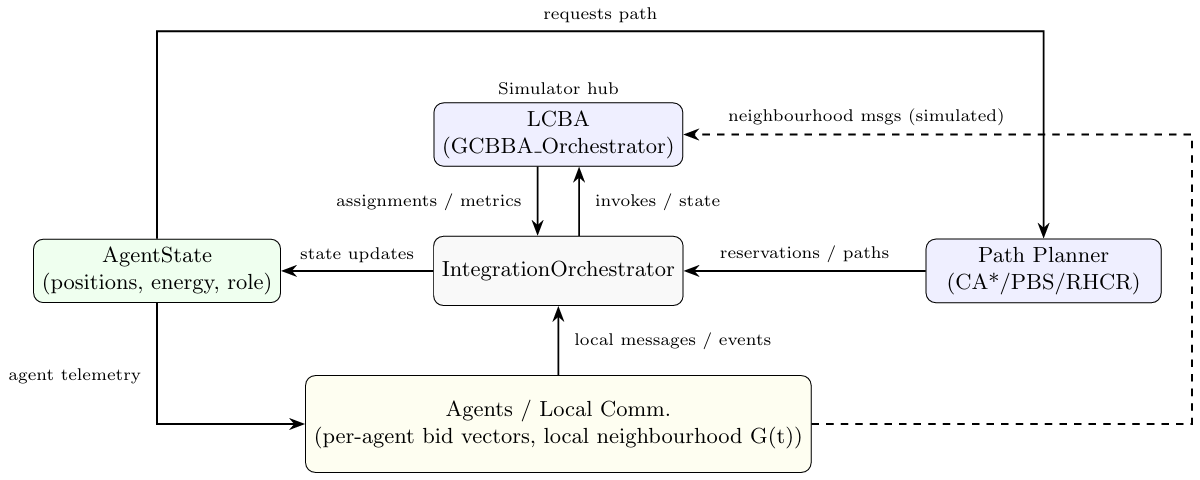
\includegraphics[width=0.9\textwidth]{figures/system_architecture}
  \textbf{[FIGURE PLACEHOLDER: System architecture block diagram showing IntegrationOrchestrator,
  GCBBA\_Orchestrator, PathPlanner, AgentState, and data flow between them.]}
  \caption{System architecture overview. The \texttt{IntegrationOrchestrator}
           coordinates the LCBA task allocator with one of three interchangeable
           path planners. Allocation is logically decentralised (agents run
           the GCBBA protocol using only local communication), while path
           planning uses a shared reservation table maintained by the
           orchestrator.}
  \label{fig:system_architecture}
\end{figure}

The task allocator runs the GCBBA/LCBA algorithm (Section~\ref{sec:method_gcbba}).
It is \emph{logically decentralised}: each agent maintains its own bid and
assignment vectors and communicates only with its current communication
neighbours.
The orchestrator simulates this communication by invoking the GCBBA update
rules for each agent using only the neighbourhood defined by $G(t)$.

The path planner (Section~\ref{sec:method_collision}) is \emph{physically
centralised} in the simulation: the orchestrator has global visibility of
all agent positions and plans collision-free paths for all agents using
a shared space-time reservation table.
% This design choice --- decentralised allocation, centralised collision
% avoidance --- is justified on two grounds.
% First, task allocation decisions are inherently private: agents in disconnected
% components have different information and may reach different allocation
% decisions, which is exactly the behaviour we wish to study.
% Second, collision-free path planning in a bounded warehouse environment does not
% require private information; centralising it eliminates the complexity of
% distributed reservation table consensus while keeping the allocation protocol
% clean for comparison across baselines.
The path planner is designed as a modular component; three implementations are
provided and studied in Section~\ref{sec:method_collision}.

Each agent's state is tracked by an \texttt{AgentState} object that records
its current position, assigned task, planned path, energy level, and charging
status.
The per-timestep simulation loop, described in
Section~\ref{sec:method_dynamic}, drives agents forward along their planned
paths and triggers replanning events as needed.


%% ── 3.3 ─────────────────────────────────────────────────────────
\section{Warehouse Environment}
\label{sec:method_environment}

Experiments are conducted across six warehouse environments of increasing scale,
summarised in Table~\ref{tab:environments}.
Each environment is a 2D gridworld with induct stations (task pickup points),
eject stations (delivery destinations), internal obstacles representing shelving
aisles, and charging stations.
All agents are initialised at their home positions at $t = 0$.

\begin{table}[htbp]
  \centering
  \caption{Warehouse environments used in the evaluation, ordered by fleet size.}
  \label{tab:environments}
  \small
  \begin{tabular}{lccccc}
    \toprule
    \textbf{Environment} & \textbf{Grid} & \textbf{Agents} $\Na$ &
    \textbf{Induct} $|\mathcal{S}^{\text{in}}|$ &
    \textbf{Eject} $|\mathcal{S}^{\text{ej}}|$ \\
    \midrule
    \texttt{warehouse\_small}  & $30\times30$   & 6   & 8  & 38 \\
    \texttt{crossdock}         & $44\times28$   & 12  & 6  & 10 \\
    \texttt{kiva}              & $36\times36$   & 20  & 5  & 10 \\
    \texttt{warehouse\_large}  & $60\times60$   & 18  & 12 & 80 \\
    \texttt{kiva\_large}       & $72\times72$   & 80  & 5  & 10 \\
    \texttt{shelf\_aisle}      & $161\times63$  & 200 & 20 & 19 \\
    \bottomrule
  \end{tabular}
\end{table}

The environments span fleet sizes from 6 to 200 agents and grid areas from
$900$ to over $10{,}000$ cells, enabling evaluation across a wide range of
congestion levels and communication graph densities.
\texttt{warehouse\_small} is used as the primary development and ablation
environment; results across all six environments are reported in the
scalability experiments (Section~\ref{sec:exp_planners}).

\begin{figure}[htbp]
  \centering
  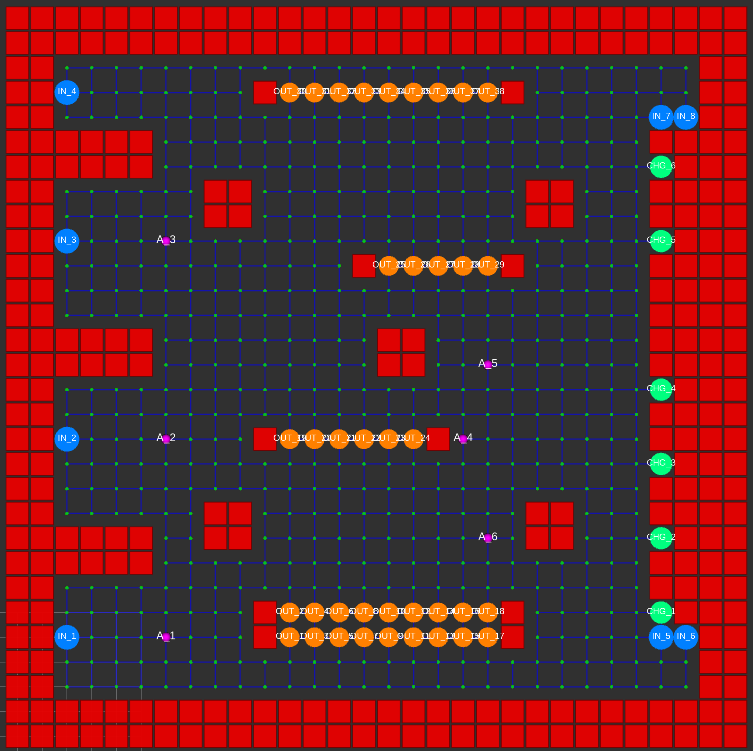
\includegraphics[width=0.6\textwidth]{figures/gridworld_warehouse_small/gridworld_warehouse_small}
  \caption{The \texttt{warehouse\_small} ($30 \times 30$) environment.
           Induct stations (blue) are task pickup locations; eject stations
           (orange) are delivery destinations; obstacles and shelving are
           shown in red; agents are shown in purple.
           Internal shelving creates constrained navigation corridors.}
  \label{fig:gridworld}
\end{figure}

\textbf{Task arrival model.}
In batch mode, all $\Nt$ tasks are injected at $t = 0$.
In steady-state mode, each induct station generates one task every
$\text{round}(1/\lambda)$ timesteps (minimum 1), where $\lambda$ is the
per-station arrival rate.
A per-station queue of depth $Q_{\max} = 5$ buffers tasks before they are
claimed by an agent; tasks that arrive when the queue is full are dropped and
counted as a capacity violation metric.

\textbf{Energy model.}
Each agent starts with full energy $E_{\max}$ and expends one unit per timestep of movement; stationary agents do not consume energy.
The charging trigger condition checks, at every timestep:
\begin{equation}
  \alpha \cdot d_{\text{charger}}(x_i(t)) > e_i(t),
  \label{eq:charge_trigger}
\end{equation}
where $e_i(t)$ is the agent's current energy level,
$d_{\text{charger}}(x_i(t))$ is the BFS shortest-path distance to the
nearest available charging station, and $\alpha \geq 1$ is the
\emph{charging trigger multiplier}.
Setting $\alpha > 1$ introduces a conservative safety margin: the agent
departs for a charger while it still holds more energy than strictly
required for the trip, preventing the degenerate case where an agent runs
out of power en route to the charger and stalls in the middle of the floor.

When the trigger fires, the agent immediately suspends its current task
(which reverts to \textsc{Planned} state and becomes eligible for reassignment),
navigates to the nearest available charging station at highest path-planning
priority, and charges at a configurable rate $\rho_c$ units per timestep
until $e_i = E_{\max}$.
Charging stations are \emph{exclusive}: at most one agent occupies each
station at a time, so the orchestrator assigns agents to distinct stations
and routes subsequent chargers to the next-nearest free station.
Once fully charged, the agent re-enters the allocation pool and a
reallocation event is triggered automatically
(Section~\ref{sec:method_triggers}).

Crucially, energy levels are also incorporated into the bid computation:
before an agent adds a task to its bundle, it checks whether the estimated
travel distance to complete that task exceeds its remaining energy budget.
If so, the task is filtered out of the candidate set.
This \emph{energy-budget filter} prevents agents from winning bids on tasks
they cannot physically complete before needing to recharge, which would
otherwise cause a mid-execution hand-off and wasted travel.

The energy configuration is validated at initialisation: if any reachable
grid position is so far from all chargers that $\alpha \cdot d > E_{\max}$,
an error is raised at startup, guaranteeing that a correctly configured
system can always reach a charger from any occupied cell.

\textbf{Wait stations.}
Idle agents --- those with no current task assignment and not en route to a
charger --- are a source of avoidable congestion: a robot parked in the
middle of a picking aisle forces every active agent to route around it,
adding detours and inflating travel times under high load.
To mitigate this, the system designates a set of \emph{wait stations}
$\mathcal{S}^{\text{wait}}$, configured in the map YAML as
\texttt{idle\_task\_stations}.
Wait stations are placed at low-traffic positions at the periphery of the
grid (typically behind induct stations or at corridor dead-ends) where
parked agents do not interrupt active delivery flows.

When an agent becomes idle and no task is immediately available, the
orchestrator routes it to its nearest unoccupied wait station using the
idle-role path planner.
Wait stations are \emph{exclusively reserved}: the orchestrator maintains a
dynamic reservation set and prevents two agents from targeting the same
station simultaneously; if all stations are occupied, the agent waits in
place.
When a new task is subsequently allocated to the waiting agent, it
immediately preempts its parking navigation and replans toward the task's
induct station, incurring no additional latency.

This behaviour mirrors industrial deployments such as Amazon Robotics and
Ocado, where idle drive units park at designated staging areas to keep main
picking aisles clear for active robots.

\textbf{Distance computation.}
All travel-time estimates used in the GCBBA bid computation
(Section~\ref{sec:method_gcbba}) are derived from BFS-precomputed shortest-path
tables over the obstacle-free grid, not Euclidean distance.
This is crucial: Euclidean distance systematically underestimates travel time
near obstacle clusters, causing agents to bid too aggressively on distant tasks
and producing suboptimal assignments.
The BFS tables are computed once at initialisation and shared across all agents.


%% ── 3.4 ─────────────────────────────────────────────────────────
\section{GCBBA for Warehouse Task Allocation}
\label{sec:method_gcbba}

The Global Consensus-Based Bundle Algorithm
(GCBBA)~\cite{kha2025enhancing} extends the Consensus-Based Bundle
Algorithm (CBBA)~\cite{choi2009consensus} in three key directions: a stronger
utility metric, a global (rather than local) consensus protocol, and a
decentralised convergence detection mechanism.
This section describes each component and then explains the additional
adaptations made to handle the warehouse setting and dynamic task arrivals,
which together constitute the Local Consensus-Based Bundle Algorithm (LCBA).


%% ── 3.4.1 ──────────────────────────────────────────────────────
\subsection{The RPT Utility Function}
\label{subsec:method_rpt}

Both CBBA and GCBBA evaluate task assignments using a score function that
must satisfy the \emph{Diminishing Marginal Gain} (DMG) property, a condition
that enables the 50\% optimality guarantee relative to the optimal assignment
value~\cite{fisher1978analysis}.

GCBBA introduces the \emph{Repeated Path Times} (RPT) utility
function~\cite{kha2025enhancing}:
\begin{equation}
  S_i^{\text{RPT}}(p_i) = -\sum_{j \in p_i}
    \tau_{ij}\!\bigl(p_i^{\preceq j}\bigr),
  \label{eq:rpt}
\end{equation}
where $p_i$ is an ordered sequence of tasks assigned to agent $i$,
$p_i^{\preceq j}$ denotes the subsequence of $p_i$ up to and including task $j$,
and $\tau_{ij}(p_i^{\preceq j})$ is the \emph{completion time} of task $j$
given that agent $i$ executes the preceding tasks in order before $j$.
In the warehouse setting, $\tau_{ij}$ is computed using the BFS-precomputed
grid distance from the agent's estimated position after completing the
preceding tasks to $s_j^{\text{in}}$, and then from $s_j^{\text{in}}$ to
$s_j^{\text{ej}}$.

Intuitively, RPT penalises both the number of tasks and their cumulative
completion time, naturally aligning the utility function with makespan
minimisation.
The marginal gain of adding task $j^*$ to an existing path $p_i$ is
\begin{equation}
  \Delta_i(j^* \mid p_i) = S_i^{\text{RPT}}(p_i \oplus j^*) - S_i^{\text{RPT}}(p_i),
  \label{eq:marginal}
\end{equation}
where $p_i \oplus j^*$ denotes optimal insertion of $j^*$ into $p_i$
(evaluated at every insertion point and taking the best).
It can be shown~\cite{kha2025enhancing} that $\Delta_i(j^* \mid p_i)$ is
non-increasing in $p_i$ under the RPT metric, confirming the DMG property.


%% ── 3.4.2 ──────────────────────────────────────────────────────
\subsection{Bundle Building Phase}
\label{subsec:method_bundle}

Each agent $i$ maintains:
a \emph{bundle} $b_i \subseteq \mathcal{T}$ (the set of tasks currently
assigned to it, unordered),
an ordered \emph{path} $p_i$ (the execution order of $b_i$),
a \emph{bid vector} $y \in \mathbb{R}^{|\mathcal{T}|}$ recording the best bid
seen for each task across all agents, and
a \emph{winner vector} $z \in \mathcal{A}^{|\mathcal{T}|}$ recording the
current winning agent for each task.

Algorithm~\ref{alg:bundle_building} describes the bundle building phase.
Each iteration, agent $i$ greedily adds the highest-marginal-gain task that it
can outbid to its bundle, up to the bundle capacity $\Lt$.
Task insertion is evaluated at every position in the current path $p_i$, with
the optimal insertion point selected.
The process terminates either when the bundle is full ($|b_i| = \Lt$), when no
task offers a positive marginal gain, or when no task can be outbid.

\begin{algorithm}[htbp]
\caption{GCBBA Bundle Building (agent $i$)}
\label{alg:bundle_building}
\begin{algorithmic}[1]
\Require Tasks $\mathcal{T}$, current path $p_i$, bid vector $y$, winner vector $z$
\Ensure Updated bundle $b_i$, path $p_i$, bids $y$, winners $z$
\While{$|b_i| < \Lt$}
  \ForAll{task $j \notin p_i$}
    \State Compute marginal gain $c_{ij} \leftarrow \Delta_i(j \mid p_i)$ via optimal insertion
  \EndFor
  \State $j^* \leftarrow \arg\max_{j \notin p_i} \bigl\{c_{ij} \;:\; c_{ij} > y_j\bigr\}$
  \If{no such $j^*$ exists} \textbf{break} \EndIf
  \State Append $j^*$ to bundle: $b_i \leftarrow b_i \cup \{j^*\}$
  \State Insert $j^*$ at optimal position in path $p_i$
  \State Update bid and winner: $y_{j^*} \leftarrow c_{ij^*}$,\; $z_{j^*} \leftarrow i$
\EndWhile
\end{algorithmic}
\end{algorithm}

In the warehouse adaptation, the BFS distance table replaces Euclidean distance
in the completion-time computation.
This ensures that $\tau_{ij}$ accurately reflects actual navigation time around
obstacles, which can differ from straight-line distance by a factor of two or
more in densely shelved environments.


%% ── 3.4.3 ──────────────────────────────────────────────────────
\subsection{Global Consensus Phase}
\label{subsec:method_consensus}

After bundle building, agents exchange their current bid and winner vectors with
their communication neighbours.
The \emph{conflict resolution rules} from~\cite{choi2009consensus,kha2025enhancing}
determine, for each task $j$ and each pair of agents $i$ and $k$, whether
agent $i$ should \textsc{Update} (accept $k$'s information), \textsc{Reset}
(remove $j$ from its own bundle), or \textsc{Leave} (retain its current
information).
The key distinction between CBBA and GCBBA lies in how many communication
rounds are performed per iteration.

CBBA performs a single round of neighbour-to-neighbour information exchange.
On a graph of diameter $D$, this means that information originating at one end
of the network may take $D$ rounds to reach the other end, during which
intermediate agents may have already committed to conflicting assignments.
As a result, CBBA is not guaranteed to produce the same assignment as SGA on
graphs with diameter greater than one.

GCBBA corrects this by performing $2D$ consensus rounds per iteration, where
$D$ is the diameter of the current communication graph~\cite{kha2025enhancing}.
After $2D$ rounds, every agent's information has propagated to every other agent
and back, guaranteeing that the final assignment is conflict-free and equivalent
to the SGA solution on connected graphs.
The diameter $D$ is estimated locally by each agent using a distributed
computation embedded in the consensus protocol.

In the LCBA extension for disconnected graphs, consensus is restricted to each
connected component of $G(t)$ independently.
Agents in different components run the consensus protocol separately and reach
self-consistent assignments within their component.
When two components reconnect at a later timestep, a reallocation is triggered
(Section~\ref{sec:method_triggers}) to resolve any cross-component conflicts.
Tasks that are still pending (not yet physically picked up) can be reassigned
at this point.


%% ── 3.4.4 ──────────────────────────────────────────────────────
\subsection{Decentralised Convergence Detection}
\label{subsec:method_convergence}

Running $2D$ consensus rounds per iteration is necessary for correctness but
computationally expensive when the graph is large or deep.
GCBBA includes a decentralised convergence detection mechanism to allow early
termination~\cite{kha2025enhancing}.

Each agent $i$ maintains a per-agent binary vector
$E^{\text{cvg}}_i \in \{0,1\}^{D+1}$, where entry $E^{\text{cvg}}_i[k] = 1$
indicates that all agents within $k$ hops of agent $i$ have converged,
i.e.\ their winner vector $z_i$ is unchanged from the previous iteration.
The first entry $E^{\text{cvg}}_i[1]$ is set by agent $i$ itself; subsequent
entries are propagated outward during the consensus rounds using neighbouring
agents' vectors.
The algorithm terminates as soon as any agent observes
$E^{\text{cvg}}_i[D+1] = 1$, which certifies that the entire network has
reached a stable assignment.
The outer iteration loop provides a fallback bound of $N_{\min} = \min(\Nt,\,\Lt\cdot\Na)$
iterations, ensuring termination even if early convergence is never detected.
Early termination significantly reduces computational cost in practice, since
convergence often occurs well before the theoretical $N_{\min}$-iteration bound.
This is especially important in the budgeted steady-state warehouse setting,
where each allocation call must complete within a per-timestep budget.


%% ── 3.4.5 ──────────────────────────────────────────────────────
\subsection{Warehouse Adaptation and LCBA}
\label{subsec:method_warehouse_adaptation}

The standard GCBBA formulation~\cite{kha2025enhancing} assumes a fixed, fully
known task set and a static communication graph.
Four adaptations are required for the warehouse setting:

\textbf{(1) Pickup-and-delivery tasks.}
Each task $\tau_j$ involves two waypoints rather than one.
The completion time $\tau_{ij}$ is computed as the BFS distance from the
agent's current position (or its projected position after completing preceding
tasks) to $s_j^{\text{in}}$, plus the BFS distance from $s_j^{\text{in}}$ to
$s_j^{\text{ej}}$.

\textbf{(2) BFS-precomputed distance tables.}
A BFS from every grid cell to every other cell is precomputed once at
initialisation and stored as a distance table.
At runtime, each call to $\tau_{ij}$ is a single table lookup, making the
marginal gain computation $O(1)$ per task rather than $O(|\mathcal{W}|)$.

\textbf{(3) Dynamic communication graph.}
The function \texttt{create\_graph\_with\_range} reconstructs $G(t)$ from
current agent positions at the start of each allocation call.
For disconnected graphs, each connected component runs the consensus protocol
independently; $D$ is taken as the maximum component diameter, ensuring every
component executes sufficient consensus rounds to converge.
The $2D$ consensus rounds are then scheduled accordingly.

\textbf{(4) Dynamic task arrivals and event-driven replanning.}
Tasks arrive online; the task set $\mathcal{T}(t)$ grows over time.
The allocation is re-invoked whenever a triggering event occurs
(Section~\ref{sec:method_triggers}).
When replanning, only tasks that have not yet been physically picked up are
eligible for reassignment, ensuring consistency with tasks already in progress.

Together, these adaptations constitute the \textbf{Local Consensus-Based Bundle
Algorithm (LCBA)}: GCBBA extended to handle disconnected and dynamically
changing communication graphs with online task arrivals.
LCBA uses the same GCBBA consensus protocol but re-invokes it on the
event-driven triggers described above, enabling continuous adaptation as tasks
arrive and communication topology evolves.


%% ── 3.5 ─────────────────────────────────────────────────────────
\section{Path Planning Strategies}
\label{sec:method_collision}

Once an allocation assigns tasks to agents, each agent must follow a
collision-free path through the warehouse grid.
The path planning component is responsible for computing these paths while
respecting the vertex and edge conflict constraints defined in
Section~\ref{sec:method_formulation}.
Three planning strategies are implemented as interchangeable modules within the
pipeline.
All three share a common interface and the same underlying space-time reservation
table, enabling fair comparisons that isolate the effect of the planning
strategy from all other system components.

A key operational feature of the pipeline is that path planners are
assigned \emph{per agent role} rather than uniformly across the fleet.
Three independent planner slots are exposed:
a \emph{task planner} for agents executing pickup-and-delivery assignments,
a \emph{charger planner} for agents navigating to a charging station, and
an \emph{idle planner} for agents navigating to a wait station.
Each slot can be configured independently to any of the three strategies
(CA*, PBS, or RHCR).
This reflects a practical insight from real warehouse deployments: the
three roles have different routing priorities and computational budgets.
Agents heading to a charger have urgent energy constraints and benefit from
the lowest-latency planner (CA*); PBS backtracking overhead is unwarranted
when a robot is nearly out of power.
Agents navigating to a wait station have no throughput urgency and can use
any lightweight planner.
Task agents are the throughput-critical path and should use the most capable
strategy the deployment can afford.
Exposing three independent slots allows practitioners to tune this
trade-off without modifying the core algorithm, and it enables the
experiments in Section~\ref{sec:exp_compact_views} to vary the task planner in
isolation while holding charger and idle routing fixed.


%% ── 3.5.1 ──────────────────────────────────────────────────────
\subsection{Space-Time Search Formulation}
\label{subsec:method_spacetime}

All planners in this pipeline operate on a space-time graph
$\mathcal{G}^{\text{ST}} = (\mathcal{V}^{\text{ST}}, \mathcal{E}^{\text{ST}})$
where each node $(x, y, t)$ represents cell $(x, y)$ at timestep $t$.
An edge connects $(x, y, t)$ to $(x', y', t+1)$ if $(x', y')$ is either the
same cell (wait action) or a cardinal neighbour of $(x, y)$ in the
obstacle-free grid.
The \emph{reservation table} $\mathcal{R}$ is a set of
$(x, y, t)$ triples indicating space-time positions reserved by agents whose
paths have already been planned.
A conflict-free path for agent $i$ must avoid all reservations in
$\mathcal{R}$ and additionally must not create edge conflicts with paths already
in $\mathcal{R}$.

The \emph{goal reservation} mechanism addresses the problem of indefinite
blocking at delivery cells: once agent $i$ arrives at its delivery cell
$s_j^{\text{ej}}$ at time $t^*$, the cell $(s_j^{\text{ej}}, t)$ is reserved
for all $t \geq t^*$ until the agent departs.
This prevents other agents from entering the cell while agent $i$ is completing
the task, while allowing the reservation to be lifted once the task is marked
complete and the agent moves on.

The heuristic used in all A*-based planners is the BFS distance from the
current cell to the goal, ignoring temporal constraints (consistent and
admissible).


%% ── 3.5.2 ──────────────────────────────────────────────────────
\subsection{Cooperative A* with Reservation Tables (CA*)}
\label{subsec:method_castar}

Cooperative A* (CA*)~\cite{silver2005cooperative} is the default planner and
the baseline against which all others are compared.
Paths are planned in two phases per replanning call.
In Phase~1, agents navigating to a charging station plan first and reserve their
paths in $\mathcal{R}$, so that task agents automatically route around them in
Phase~2.
Within each phase, the planning order is randomised to avoid systematic priority
bias: no agent consistently receives the easiest routing problem by virtue of a
fixed priority assignment.
Idle agents (no current goal) are handled outside the main planning loop by
holding their current position in $\mathcal{R}$ so that active agents plan
around them.

Each agent plans a shortest path through the space-time graph subject to the
reservations already in $\mathcal{R}$, adds its own planned positions, and the
next agent plans around all accumulated reservations.
The space-time A* search uses a BFS-precomputed obstacle-aware distance table
as the heuristic, which is admissible and tighter than Manhattan distance in
cluttered warehouse layouts.

CA* is complete under the fixed reservation constraints if the space-time graph
is finite (i.e.\ there is always a sequence of wait actions that allows an agent
to eventually reach its goal without conflicting with higher-priority agents).
In practice, the random planning order does not guarantee completeness: a given
ordering can leave a low-priority agent unable to reach its goal because earlier
agents permanently block all routes.
The stuck-detection mechanism described in
Section~\ref{subsec:method_stuck} provides a practical recovery path by
triggering path replanning when an agent fails to make progress.

CA* has time complexity $O(n \cdot |\mathcal{W}| \cdot T)$ per planning
call, where $n$ is the number of agents being planned for and $T$ is the
planning horizon.
It is the most computationally efficient of the three planners when the
number of conflicts is low, since each agent requires only a single A*
pass with no backtracking or constraint propagation.


%% ── 3.5.3 ──────────────────────────────────────────────────────
\subsection{Priority-Based Search (PBS)}
\label{subsec:method_pbs}

Priority-Based Search (PBS) extends the CA* idea by relaxing the fixed
priority order.
Rather than assigning priorities a priori, PBS attempts to find a conflict-free
set of paths by dynamically resolving conflicts that arise during planning.
When two agents $i$ and $j$ produce conflicting paths, PBS introduces a
priority constraint ($i > j$ or $j > i$) and replans the lower-priority agent's
path subject to that constraint.
If the constraint leads to a dead end, PBS backtracks and tries the alternative
priority ordering.

PBS is complete under the assumption that a conflict-free solution exists.
In practice, PBS tends to produce slightly shorter aggregate paths than CA*
because it can reassign priorities to avoid unnecessary detours, at the cost of
a higher worst-case planning time.
For the primary development environment ($\Na = 6$, \texttt{warehouse\_small}),
the difference between CA* and PBS in both path quality and computation time is modest.


%% ── 3.5.4 ──────────────────────────────────────────────────────
\subsection{Rolling Horizon Collision Resolution (RHCR)}
\label{subsec:method_rhcr}

Rolling Horizon Collision Resolution (RHCR), introduced by
\citet{li2021lifelong} for lifelong MAPF in large warehouses, addresses the
computational challenge of planning for many agents over long horizons by
restricting attention to a sliding time window.

RHCR is parameterised by a \emph{window size} $w$ (the number of timesteps
ahead to plan) and a \emph{replanning period} $h \leq w$ (the number of
timesteps to execute before replanning).
At each replanning event, all agents plan paths for the next $w$ timesteps
using the chosen inner solver (CA* in the RHCR variant).
After $h$ timesteps of execution, paths are replanned for the next window.
Setting $h = w$ causes replanning only when the window is exhausted; setting
$h < w$ enables more frequent replanning that can react to task completions
and allocation changes within the window.

RHCR decouples planning complexity from the total mission horizon: even if the
full mission spans thousands of timesteps, each planning call only considers
$w$ timesteps.
This is particularly beneficial in the ceiling-aware steady-state setting,
where missions have no defined end.
The trade-off is that plans may be suboptimal near the window boundary, as
agents cannot anticipate conflicts that arise just beyond $t + w$.


%% ── 3.5.5 ──────────────────────────────────────────────────────
\subsection{Planner Comparison}
\label{subsec:method_planner_comparison}

Table~\ref{tab:planner_comparison} summarises the three planners along four
dimensions: completeness, optimality criterion, asymptotic time complexity per
planning call, and scalability.

\begin{table}[htbp]
  \centering
  \caption{Comparison of the three path planning strategies.
           $n$ = number of agents, $|\mathcal{W}|$ = number of free cells,
           $T$ = planning horizon, $w$ = rolling window size.}
  \label{tab:planner_comparison}
  \small
  \begin{tabular}{lcccc}
    \toprule
    \textbf{Planner} & \textbf{Complete} & \textbf{Optimal} &
    \textbf{Complexity} & \textbf{Scale} \\
    \midrule
    CA*   & Practical & No & $O(n \cdot |\mathcal{W}| \cdot T)$ & $\leq$30 agents \\
    PBS   & Yes       & No & $O(n! \cdot |\mathcal{W}| \cdot T)$ worst & $\leq$30 agents \\
    RHCR  & Practical & No & $O(n \cdot |\mathcal{W}| \cdot w)$ & $\leq$100 agents \\
    \bottomrule
  \end{tabular}
\end{table}

A key architectural advantage of the system is that the path planner is a
configurable parameter of the \texttt{IntegrationOrchestrator}: any allocation
method (LCBA, CBBA, SGA, or DMCHBA) can be paired with any of the three
planners without modification.
For the allocation comparison experiments (Sections~\ref{sec:exp_batch} and
\ref{sec:exp_steady_state}), CA* is held fixed across all methods as an
experimental control to isolate the effect of the allocation algorithm.
Section~\ref{sec:exp_compact_views} presents the batch compact-view summaries
used to compare planner behaviour across maps; a dedicated planner comparison
section is in preparation.


%% ── 3.6 ─────────────────────────────────────────────────────────
\section{Dynamic Replanning via the Integration Orchestrator}
\label{sec:method_dynamic}


%% ── 3.6.1 ──────────────────────────────────────────────────────
\subsection{Simulation Loop and Task Lifecycle}
\label{subsec:method_loop}

The \texttt{IntegrationOrchestrator} drives the simulation through a
per-timestep loop.
At each timestep $t$, the following operations are executed in order:
\begin{enumerate}
  \item \textbf{Task injection.}
        In steady-state mode, each induct station injects a task when at least
        $\Delta_{\lambda} = \text{round}(1/\lambda)$ timesteps have elapsed
        since its last injection, provided its queue depth is below $Q_{\max}$.
        Newly injected tasks are added to the pending task set
        $\mathcal{T}_{\text{pending}}(t)$.
  \item \textbf{Allocation trigger check.}
        The orchestrator checks whether any allocation trigger condition is
        met (Section~\ref{sec:method_triggers}).
        If so, the LCBA algorithm is invoked.
  \item \textbf{Path planning.}
        For each agent whose path is stale (flagged by
        \texttt{needs\_new\_path}), a new collision-free path is computed
        using the chosen path planner.
  \item \textbf{Agent execution.}
        Each agent advances one step along its planned path.
        If an agent reaches $s_j^{\text{in}}$ while $\tau_j$ is in
        state \textsc{Planned}, the task transitions to
        \textsc{Executing}.
        If the agent subsequently reaches $s_j^{\text{ej}}$, the task
        transitions to \textsc{Completed}.
  \item \textbf{Energy management.}
        Agents with low energy are directed to charging stations.
        Charging state changes trigger an allocation rerun.
  \item \textbf{Metrics recording.}
        Per-timestep metrics (queue depths, agent positions, task states)
        are recorded.
\end{enumerate}

The three-state task lifecycle (\textsc{Planned} $\to$ \textsc{Executing}
$\to$ \textsc{Completed}) is central to conflict resolution in LCBA.
Only \textsc{Planned} tasks can be reassigned by a subsequent allocation call;
once a task is \textsc{Executing} (agent is en route to the eject station),
it is locked to that agent and cannot be reallocated.
This prevents the degenerate case where an agent drops a task mid-execution
because a competing agent bid higher on it during a reallocation.


%% ── 3.6.2 ──────────────────────────────────────────────────────
\subsection{Allocation Trigger Conditions}
\label{sec:method_triggers}

The LCBA allocation is invoked under five conditions, listed in priority order:

\begin{enumerate}
  \item \textbf{Initialisation.} At $t = 0$ (or after a system reset),
        allocation always runs.
  \item \textbf{Charging state change.} When an agent starts or finishes
        charging, its available capacity changes, justifying immediate
        reallocation.
  \item \textbf{New tasks and idle agents.} If new tasks have been injected
        into $\mathcal{T}_{\text{pending}}$ and at least one agent is idle,
        allocation is triggered immediately to minimise task wait time.
  \item \textbf{Batch completion threshold.} If at least
        $\max(2, \lfloor \Na/3 \rfloor)$ tasks have been completed since
        the last allocation, and a cooldown of
        $\max(3, \lfloor r_{\text{interval}}/3 \rfloor)$ timesteps has
        elapsed, allocation is triggered.
        The batch threshold prevents excessive replanning when tasks complete
        in rapid succession; the cooldown prevents thrashing.
  \item \textbf{Idle agents with pending tasks.}
        If idle agents exist and pending tasks are waiting, allocation is
        triggered after the cooldown period, ensuring that agents do not sit
        idle while work is available.
\end{enumerate}

Triggering conditions 3--5 are subject to the cooldown, which limits the
replanning rate and avoids the computational cost of running LCBA at every
timestep.
The value $r_{\text{interval}} = 50$ timesteps is the canonical cooldown used
in the dynamic experiments; Section~\ref{sec:exp_sensitivity} evaluates
sensitivity to this choice.


%% ── 3.6.3 ──────────────────────────────────────────────────────
\subsection{The Rerun Interval as a Fallback Trigger}
\label{subsec:method_rerun_interval}

LCBA is inherently event-driven: allocation is triggered by task completions,
charging state changes, and idle-agent conditions
(Section~\ref{sec:method_triggers}).
In practice these events fire frequently enough that periodic time-based
reallocation is unnecessary under normal operation.
The \emph{rerun interval} $r_{\text{interval}}$ serves purely as a
\emph{safety-net fallback}: if none of the primary triggers have fired for
$r_{\text{interval}}$ timesteps and pending tasks exist, allocation runs
regardless.
This prevents the degenerate case where all agents are simultaneously in
transit (no completions, no idle agents) and a newly injected task stalls
indefinitely.

Section~\ref{sec:exp_sensitivity} presents a sensitivity sweep over
$r_{\text{interval}}$ and confirms that performance is insensitive to the
exact value within a wide range, validating the canonical choice of
$r_{\text{interval}} = 50$ timesteps.


%% ── 3.6.4 ──────────────────────────────────────────────────────
\subsection{Stuck Agent Detection and Recovery}
\label{subsec:method_stuck}

An agent is classified as \emph{stuck} when its position has not changed for
$\theta_{\text{stuck}} = 15$ consecutive timesteps while it holds a task
assignment.
This condition detects situations where the path planner has assigned a path
that the agent cannot execute due to a persistent conflict with a
higher-priority agent. This is a failure mode that arises in priority-based planners
when priorities create a cyclic dependency.

When an agent is detected as stuck, its \texttt{needs\_new\_path} flag is set,
triggering path replanning at the next timestep.
Crucially, stuck detection does \emph{not} trigger a full LCBA rerun: the
computational cost of rerunning the full consensus protocol is not warranted
when the underlying assignment is still valid.
Replanning the path alone, with the stuck agent's priority temporarily elevated,
is sufficient to break the deadlock in the vast majority of cases observed
during evaluation.


%% ── 3.7 ─────────────────────────────────────────────────────────
\section{Baseline Methods}
\label{sec:method_baselines}

Three baseline allocation algorithms are compared against LCBA.
Because the path planner is a configurable, interchangeable component, any
baseline can be evaluated with any of the three planners.
For the allocation comparison experiments the planner is held fixed at CA*
across all methods, using the same \texttt{IntegrationOrchestrator}
infrastructure, so that any performance differences are attributable solely to
the allocation strategy.

\textbf{Sequential Greedy Algorithm (SGA).}
SGA is the centralised optimality reference.
At each allocation call, SGA iterates over all (agent, task) pairs in
descending order of marginal gain and greedily assigns each task to the best
available agent, updating each agent's projected position before the next
assignment.
SGA achieves the 50\%-optimality guarantee under DMG
utilities~\cite{fisher1978analysis} --- that is, SGA's assignment value is
guaranteed to be at least 50\% of the optimal assignment value.
On disconnected graphs, SGA runs independently within each connected component,
which is a generous assumption --- a centralised algorithm would, in practice,
have no knowledge of the existence or content of isolated components.
This makes SGA a conservative upper bound on achievable performance.
SGA does not replan between allocation calls; it is re-invoked at the same
triggering events as LCBA for a fair comparison.

\textbf{Consensus-Based Bundle Algorithm (CBBA).}
CBBA~\cite{choi2009consensus} is the direct predecessor of GCBBA.
It uses the same bundle building procedure as LCBA but replaces the $2D$-round
global consensus with a single round of local information exchange.
This makes CBBA computationally cheaper per call but at the cost of convergence
guarantees on non-fully-connected graphs.
CBBA is evaluated in its static configuration (allocation at $t=0$ only),
consistent with its original design for batch task settings.
Dynamic CBBA is not evaluated separately since CBBA's local consensus already
prevents it from correctly resolving conflicts that span disconnected components,
making dynamic reallocation less meaningful.

\textbf{Distributed Matching by Clone Hungarian-Based Algorithm (DMCHBA).}
DMCHBA~\cite{samiei2024dmchba} is a state-of-the-art decentralised task
allocation method based on distributed Hungarian matching.
It is included as the primary competing baseline from recent literature.
DMCHBA provides strong performance guarantees on connected graphs but, like
CBBA, has not been designed for the dynamic, disconnected communication
settings that characterise the LCBA evaluation.


%% ── 3.8 ─────────────────────────────────────────────────────────
\section{Design Decisions and Rationale}
\label{sec:method_design}

This section explicitly names the key design choices and the rationale behind
each, to aid reproducibility and to anticipate questions about the scope of
the experimental evaluation.

\textbf{Hybrid decentralised allocation / centralised path planning.}
As argued in Section~\ref{sec:method_overview}, task allocation is kept
decentralised to faithfully model communication constraints, while path planning
is centralised to avoid the added complexity of distributed reservation table
synchronisation.
This is a deliberate choice to isolate the allocation variable in experiments.
A fully decentralised path planner (such as distributed PIBT) would be an
interesting extension but is out of scope for this thesis.

\textbf{Batch-threshold replanning triggers over fixed-interval.}
A fixed-interval replanning trigger (every $k$ timesteps) would cause
unnecessary reallocation when no task completions have occurred, and would
delay reallocation when many tasks complete in a burst.
The batch-threshold trigger (Section~\ref{sec:method_triggers}) is more
responsive: it fires as soon as enough state has changed to justify the
computational cost of a full LCBA run.

\textbf{BFS distance tables over Euclidean distance.}
Euclidean distance is $O(1)$ to compute but systematically incorrect in
shelved environments.
The one-time $O(|\mathcal{W}|^2)$ BFS precomputation pays for itself
immediately: bid computation for all subsequent timesteps is $O(1)$
per (agent, task) pair with accurate distances, compared to $O(|\mathcal{W}|)$
per pair for on-demand shortest-path computation.

\textbf{Maximum component diameter for disconnected graphs.}
Using the maximum diameter across all components ensures that the consensus
protocol converges within each component.
An alternative --- using the diameter of the largest component only --- would
fail to converge in small isolated components whose diameter exceeds the
planned number of consensus rounds.

\textbf{Goal reservation without unlimited future locking.}
Reserving a delivery cell only from the agent's arrival time until task
completion (rather than reserving it indefinitely) allows other agents to pass
through the cell after the task is marked complete.
Unlimited locking was tested early in development and caused unnecessary
detours that degraded throughput by up to 15\% in high-load configurations.

\textbf{Energy-budget filtering as a first-class allocation constraint.}
Filtering tasks that exceed an agent's remaining energy budget during bundle
building adds one distance comparison per (agent, task) pair --- negligible
computational cost --- but prevents a qualitatively important failure mode.
Without the filter, an agent could win a bid on a task, trigger the charging
threshold partway to the induct station, suspend execution, and leave the
task re-queued and delayed.
By excluding unaffordable tasks at bid time, LCBA ensures that every winning
bid corresponds to a task the agent can physically complete in its current
energy state.

\textbf{Wait stations over in-place idling.}
The simpler alternative --- leaving idle agents in place when no task is
available --- produces unpredictable blockages.
In high-load configurations, agents that complete a delivery at a popular
eject station will hold position there, blocking subsequent deliveries to the
same cell and forcing detours.
Wait stations displace idle agents to pre-configured low-traffic positions,
decoupling the delivery cell from the parking problem and reducing the
expected path length of active agents by eliminating the most common
sources of in-aisle obstruction.

\textbf{Operational realism as an evaluation criterion.}
Most academic MAPF benchmarks assume infinite-energy agents that can park
anywhere in the grid.
This thesis deliberately breaks both assumptions: agents have finite energy
(requiring proactive charging), and idle agents are confined to designated
wait stations (limiting congestion).
The goal is not to claim that specific parameter values
($E_{\max}$, $\alpha$, $|\mathcal{S}^{\text{wait}}|$) match any particular
deployment, but to ensure that the qualitative constraint structure
matches real systems --- so that algorithmic design choices (energy-budget
filtering, charging-triggered reallocation, role-separated planners)
are exercised under realistic operational pressure rather than evaluated
in an artificially simplified setting.

%% ============================================================
%%  Chapter 4: Experimental Evaluation
%% ============================================================
\chapter{Experimental Evaluation}
\label{chap:experiments}

% GUIDANCE: 15--20 pages. This is your results chapter.
% Write the setup sections NOW (they don't need results).
% Leave \todo placeholders for figures and tables.
% Fill in numbers once experiments finish.


% ── 4.1 ─────────────────────────────────────────────────────────
\section{Experimental Setup}
\label{sec:exp_setup}


\subsection{Environment Configuration}
\label{subsec:exp_environment}

All experiments are run in the same warehouse gridworld simulation stack,
with map-specific geometry, agent count, induct stations, and eject stations
loaded from YAML configuration files. One simulation timestep corresponds to
one discrete planning/execution update in the environment. Unless otherwise
noted, all allocation methods share the same downstream path-planning and
collision-avoidance pipeline to isolate the effect of task-allocation logic.


\subsection{Parameters Swept}
\label{subsec:exp_parameters}

All experiments sweep the following parameters:

\begin{itemize}
  \item \textbf{Communication range} is map-scaled from diagonal fractions
    $\{0.1, 0.2, 0.35, 0.6, 1.2\}$ and rounded to grid units.
  \item \textbf{Batch tasks per induct station} in full mode:
    $\{8, 10, 12, 15\}$ (reliability-first sweep).
  \item \textbf{Batch tasks per induct station} in stress mode:
    $\{10, 20, 30, 40\}$ (overload analysis, reported separately).
  \item \textbf{Steady-state arrival fractions} in full mode:
    $\{0.25, 0.4, 0.55, 0.7, 0.85\}$ times the map-specific
    estimated steady-state capacity.
  \item \textbf{Steady-state arrival fractions} in quick mode:
    $\{0.5, 0.8\}$ times the map-specific estimated steady-state capacity.
  \item \textbf{Steady-state arrival fractions} in stress mode:
    $\{0.6, 0.8, 1.0, 1.2, 1.4\}$ times the map-specific estimated
    steady-state capacity.
  \item \textbf{Rerun interval} (Dynamic GCBBA only)
        $\in \{10, 25, 50, 100, 200\}$ timesteps, with $ri = 50$
        as the canonical configuration.
\end{itemize}

Each configuration is repeated across two random seeds ($42$, $123$) in full mode.
The maximum timestep budget is 1500 for steady-state and 3000 for batch runs.

For steady-state experiments, quick mode is now a low-load smoke check,
full mode is intentionally conservative so that the main thesis figures focus on
stable operating regions, and stress mode is reserved for overload behavior.

A complete sweep-count table is omitted here for brevity and will be added in
the final manuscript revision after steady-state result integration.


\subsection{Batch Reliability Screening Across Maps}
\label{subsec:exp_batch_reliability_screen}

To ensure that the main thesis comparisons are based on stable operating regimes,
we screened each map using the latest full-mode batch runs and marked a load point
as \emph{reliable} when the wall-clock timeout rate was at most $20\%$.

Table~\ref{tab:batch_reliability_screen} summarizes the maximum reliable batch load
per map and the recommended reporting role in this thesis.

\begin{table}[htbp]
  \centering
  \small
  \caption{Batch reliability screen from full-mode runs. A map is marked
       as main-analysis-ready when it provides usable low-to-mid load
       comparisons without timeout-dominated behavior.}
  \label{tab:batch_reliability_screen}
  \begin{tabular}{lccc}
    \hline
    Map & Max reliable task count & Completed-only makespan usable & Recommended use \\
    \hline
    gridworld\_crossdock       & 90  & Yes & Main analysis \\
    gridworld\_warehouse\_small & 120 & Partial (best at lower loads) & Main analysis \\
    gridworld\_warehouse\_large & 144 & Partial (exclude top load in main) & Main analysis \\
    gridworld\_kiva            & 75  & No (timestep-ceiling dominated) & Secondary / partial-completion \\
    gridworld\_kiva\_large      & N/A & No & Stress / appendix \\
    gridworld\_shelf\_aisle      & N/A & No & Stress / appendix \\
    \hline
  \end{tabular}
\end{table}

The resulting presentation policy is: (i) use crossdock, warehouse\_small,
and warehouse\_large as the primary cross-map batch comparison set,
(ii) report kiva primarily through completion-fraction and timeout behavior,
and (iii) treat kiva\_large and shelf\_aisle as stress-test regimes.

The compact batch figures used for this screening were generated from:
\begin{itemize}
  \item \texttt{results/experiments/gridworld\_warehouse\_small/20260425\_012846/batch\_results/compact\_views/}
  \item \texttt{results/experiments/gridworld\_crossdock/20260425\_022224/batch\_results/compact\_views/}
  \item \texttt{results/experiments/gridworld\_kiva/20260425\_030403/batch\_results/compact\_views/}
  \item \texttt{results/experiments/gridworld\_warehouse\_large/20260425\_044219/batch\_results/compact\_views/}
  \item \texttt{results/experiments/gridworld\_kiva\_large/20260425\_062503/batch\_results/compact\_views/}
  \item \texttt{results/experiments/gridworld\_shelf\_aisle/20260425\_074507/batch\_results/compact\_views/}
\end{itemize}

For each run, the primary reliability visuals are:
\texttt{compact\_heatmap\_completion\_rate.png},
\texttt{compact\_heatmap\_timeout\_rate.png},
\texttt{compact\_capacity\_curve.png}, and
\texttt{compact\_completion\_degradation\_by\_comm\_range.png}.
When available, completed-only makespan is shown via
\texttt{compact\_makespan\_completed\_by\_comm\_range.png}.

\subsubsection*{Main-Map Reliability Figures}

\begin{figure}[htbp]
  \centering
  \begin{subfigure}[t]{0.32\textwidth}
    \centering
    
\includegraphics[width=\textwidth]{../results/experiments/gridworld_crossdock/20260425_022224/batch_results/compact_views/compact_heatmap_completion_rate.png}
    \caption{Crossdock}
  \end{subfigure}
  \hfill
  \begin{subfigure}[t]{0.32\textwidth}
    \centering
    
\includegraphics[width=\textwidth]{../results/experiments/gridworld_warehouse_small/20260425_012846/batch_results/compact_views/compact_heatmap_completion_rate.png}
    \caption{Warehouse-small}
  \end{subfigure}
  \hfill
  \begin{subfigure}[t]{0.32\textwidth}
    \centering
    
\includegraphics[width=\textwidth]{../results/experiments/gridworld_warehouse_large/20260425_044219/batch_results/compact_views/compact_heatmap_completion_rate.png}
    \caption{Warehouse-large}
  \end{subfigure}
  \caption{Completion-rate heatmaps for the three main-analysis maps used in the batch reliability screen.}
  \label{fig:batch_completion_heatmaps_main_maps}
\end{figure}

\begin{figure}[htbp]
  \centering
  \begin{subfigure}[t]{0.32\textwidth}
    \centering
    
\includegraphics[width=\textwidth]{../results/experiments/gridworld_crossdock/20260425_022224/batch_results/compact_views/compact_heatmap_timeout_rate.png}
    \caption{Crossdock}
  \end{subfigure}
  \hfill
  \begin{subfigure}[t]{0.32\textwidth}
    \centering
    
\includegraphics[width=\textwidth]{../results/experiments/gridworld_warehouse_small/20260425_012846/batch_results/compact_views/compact_heatmap_timeout_rate.png}
    \caption{Warehouse-small}
  \end{subfigure}
  \hfill
  \begin{subfigure}[t]{0.32\textwidth}
    \centering
    
\includegraphics[width=\textwidth]{../results/experiments/gridworld_warehouse_large/20260425_044219/batch_results/compact_views/compact_heatmap_timeout_rate.png}
    \caption{Warehouse-large}
  \end{subfigure}
  \caption{Timeout-rate heatmaps for main-analysis maps. Low-to-mid loads are stable, while top loads show map-dependent degradation.}
  \label{fig:batch_timeout_heatmaps_main_maps}
\end{figure}

\begin{figure}[htbp]
  \centering
  \begin{subfigure}[t]{0.32\textwidth}
    \centering
    
\includegraphics[width=\textwidth]{../results/experiments/gridworld_crossdock/20260425_022224/batch_results/compact_views/compact_capacity_curve.png}
    \caption{Crossdock}
  \end{subfigure}
  \hfill
  \begin{subfigure}[t]{0.32\textwidth}
    \centering
    
\includegraphics[width=\textwidth]{../results/experiments/gridworld_warehouse_small/20260425_012846/batch_results/compact_views/compact_capacity_curve.png}
    \caption{Warehouse-small}
  \end{subfigure}
  \hfill
  \begin{subfigure}[t]{0.32\textwidth}
    \centering
    
\includegraphics[width=\textwidth]{../results/experiments/gridworld_warehouse_large/20260425_044219/batch_results/compact_views/compact_capacity_curve.png}
    \caption{Warehouse-large}
  \end{subfigure}
  \caption{Critical-load frontier curves (completion threshold $\geq 0.95$) for main-analysis maps.}
  \label{fig:batch_capacity_main_maps}
\end{figure}

\begin{figure}[htbp]
  \centering
  \begin{subfigure}[t]{0.32\textwidth}
    \centering
    
\includegraphics[width=\textwidth]{../results/experiments/gridworld_crossdock/20260425_022224/batch_results/compact_views/compact_completion_degradation_by_comm_range.png}
    \caption{Crossdock}
  \end{subfigure}
  \hfill
  \begin{subfigure}[t]{0.32\textwidth}
    \centering
    
\includegraphics[width=\textwidth]{../results/experiments/gridworld_warehouse_small/20260425_012846/batch_results/compact_views/compact_completion_degradation_by_comm_range.png}
    \caption{Warehouse-small}
  \end{subfigure}
  \hfill
  \begin{subfigure}[t]{0.32\textwidth}
    \centering
    
\includegraphics[width=\textwidth]{../results/experiments/gridworld_warehouse_large/20260425_044219/batch_results/compact_views/compact_completion_degradation_by_comm_range.png}
    \caption{Warehouse-large}
  \end{subfigure}
  \caption{Completion-vs-load degradation curves by communication range for main-analysis maps. These plots show graceful vs sharp degradation regimes and support the load-screening decisions in Table~\ref{tab:batch_reliability_screen}.}
  \label{fig:batch_degradation_main_maps}
\end{figure}

\begin{figure}[htbp]
  \centering
  \begin{subfigure}[t]{0.32\textwidth}
    \centering
    
\includegraphics[width=\textwidth]{../results/experiments/gridworld_crossdock/20260425_022224/batch_results/compact_views/compact_tradeoff.png}
    \caption{Crossdock}
  \end{subfigure}
  \hfill
  \begin{subfigure}[t]{0.32\textwidth}
    \centering
    
\includegraphics[width=\textwidth]{../results/experiments/gridworld_warehouse_small/20260425_012846/batch_results/compact_views/compact_tradeoff.png}
    \caption{Warehouse-small}
  \end{subfigure}
  \hfill
  \begin{subfigure}[t]{0.32\textwidth}
    \centering
    
\includegraphics[width=\textwidth]{../results/experiments/gridworld_warehouse_large/20260425_044219/batch_results/compact_views/compact_tradeoff.png}
    \caption{Warehouse-large}
  \end{subfigure}
  \caption{Completion-versus-wall-time tradeoff for main-analysis maps. Pareto-favorable regions correspond to high completion at lower wall-time.}
  \label{fig:batch_tradeoff_main_maps}
\end{figure}

\subsubsection*{Stress-Regime Figures}

\begin{figure}[htbp]
  \centering
  \begin{subfigure}[t]{0.32\textwidth}
    \centering
    
\includegraphics[width=\textwidth]{../results/experiments/gridworld_kiva/20260425_030403/batch_results/compact_views/compact_heatmap_timeout_rate.png}
    \caption{Kiva (secondary)}
  \end{subfigure}
  \hfill
  \begin{subfigure}[t]{0.32\textwidth}
    \centering
    
\includegraphics[width=\textwidth]{../results/experiments/gridworld_kiva_large/20260425_062503/batch_results/compact_views/compact_heatmap_timeout_rate.png}
    \caption{Kiva-large (stress)}
  \end{subfigure}
  \hfill
  \begin{subfigure}[t]{0.32\textwidth}
    \centering
    
\includegraphics[width=\textwidth]{../results/experiments/gridworld_shelf_aisle/20260425_074507/batch_results/compact_views/compact_heatmap_timeout_rate.png}
    \caption{Shelf-aisle (stress)}
  \end{subfigure}
  \caption{Timeout-rate heatmaps for secondary/stress maps. These are interpreted as robustness stress regimes rather than primary efficiency comparisons.}
  \label{fig:batch_timeout_heatmaps_stress_maps}
\end{figure}

\subsubsection*{Steady-State Figures (Rolling Integration)}

Steady-state results are being integrated incrementally as map runs finish.
At this revision, \texttt{gridworld\_warehouse\_small} and
\texttt{gridworld\_crossdock} are available as the current stable-regime SS maps,
and \texttt{gridworld\_kiva} is now available as a stress-regime SS map.
The SS thesis presentation uses the same compact-view structure across maps:
throughput, wait-time, capacity frontier, and completion progress split by stop
reason.

The newest steady-state runs are more representative than the earlier warm-started
versions: warehouse-small now completes more cleanly with much lower wait time,
while crossdock still shows timeout pressure but with substantially less wall-clock
domination than before. Kiva remains ceiling-dominated, so it is interpreted as a
stress-regime robustness case rather than a stable-regime efficiency comparison.
The saturation early-stop did not trigger in these maps, so the current
improvement comes from the revised arrival policy rather than from aggressive
early termination.

Current steady-state compact-view path:
\begin{itemize}
  \item \texttt{results/experiments/gridworld\_warehouse\_small/20260426\_135556/ss\_results/compact\_views/}
  \item \texttt{results/experiments/gridworld\_crossdock/20260426\_141042/ss\_results/compact\_views/}
  \item \texttt{results/experiments/gridworld\_kiva/20260426\_195056/ss\_results/compact\_views/}
\end{itemize}

\begin{figure}[htbp]
  \centering
  \begin{subfigure}[t]{0.48\textwidth}
    \centering
    
\includegraphics[width=\textwidth]{../results/experiments/gridworld_warehouse_small/20260426_135556/ss_results/compact_views/compact_heatmap_throughput.png}
    \caption{Warehouse-small: throughput}
  \end{subfigure}
  \hfill
  \begin{subfigure}[t]{0.48\textwidth}
    \centering
    
\includegraphics[width=\textwidth]{../results/experiments/gridworld_warehouse_small/20260426_135556/ss_results/compact_views/compact_heatmap_wait_time.png}
    \caption{Warehouse-small: wait time}
  \end{subfigure}

  \vspace{0.7em}

  \begin{subfigure}[t]{0.48\textwidth}
    \centering
    
\includegraphics[width=\textwidth]{../results/experiments/gridworld_crossdock/20260426_141042/ss_results/compact_views/compact_heatmap_throughput.png}
    \caption{Crossdock: throughput}
  \end{subfigure}
  \hfill
  \begin{subfigure}[t]{0.48\textwidth}
    \centering
    
\includegraphics[width=\textwidth]{../results/experiments/gridworld_crossdock/20260426_141042/ss_results/compact_views/compact_heatmap_wait_time.png}
    \caption{Crossdock: wait time}
  \end{subfigure}
  \caption{Steady-state throughput and wait-time heatmaps for the currently completed SS maps.}
  \label{fig:ss_throughput_wait_heatmaps_current_maps}
\end{figure}

\begin{figure}[htbp]
  \centering
  \begin{subfigure}[t]{0.48\textwidth}
    \centering
    
\includegraphics[width=\textwidth]{../results/experiments/gridworld_warehouse_small/20260426_135556/ss_results/compact_views/compact_capacity_curve.png}
    \caption{Warehouse-small}
  \end{subfigure}
  \hfill
  \begin{subfigure}[t]{0.48\textwidth}
    \centering
    
\includegraphics[width=\textwidth]{../results/experiments/gridworld_crossdock/20260426_141042/ss_results/compact_views/compact_capacity_curve.png}
    \caption{Crossdock}
  \end{subfigure}
  \caption{Steady-state capacity frontier for the currently completed SS maps.}
  \label{fig:ss_capacity_current_maps}
\end{figure}

\begin{figure}[htbp]
  \centering
  \begin{subfigure}[t]{0.48\textwidth}
    \centering
    
\includegraphics[width=\textwidth]{../results/experiments/gridworld_warehouse_small/20260426_135556/ss_results/compact_views/compact_completion_progress_all_tasks_completed.png}
    \caption{Warehouse-small}
  \end{subfigure}
  \hfill
  \begin{subfigure}[t]{0.48\textwidth}
    \centering
    
\includegraphics[width=\textwidth]{../results/experiments/gridworld_crossdock/20260426_141042/ss_results/compact_views/compact_completion_progress_all_tasks_completed.png}
    \caption{Crossdock}
  \end{subfigure}
  \caption{Steady-state completion progress for runs that finished all tasks.}
  \label{fig:ss_completion_progress_completed_current_maps}
\end{figure}

\begin{figure}[htbp]
  \centering
  \begin{subfigure}[t]{0.48\textwidth}
    \centering
    
\includegraphics[width=\textwidth]{../results/experiments/gridworld_warehouse_small/20260426_135556/ss_results/compact_views/compact_completion_progress_timestep_ceiling.png}
    \caption{Warehouse-small}
  \end{subfigure}
  \hfill
  \begin{subfigure}[t]{0.48\textwidth}
    \centering
    
\includegraphics[width=\textwidth]{../results/experiments/gridworld_crossdock/20260426_141042/ss_results/compact_views/compact_completion_progress_timestep_ceiling.png}
    \caption{Crossdock}
  \end{subfigure}
  \caption{Steady-state completion progress for runs that reached the timestep ceiling.}
  \label{fig:ss_completion_progress_timestep_ceiling_current_maps}
\end{figure}

\paragraph{Kiva Stress-Regime Steady-State Insertion.}
The latest Kiva steady-state run is included as a stress-regime result.
Kiva does not currently produce a completed-runs progress panel in this run
because the completed stop reason is absent; therefore, the chapter reports
throughput/wait heatmaps, capacity frontier, and timestep-ceiling completion progress.
This run is useful for robustness interpretation, but it should not be read as a
real-time control benchmark.

\begin{figure}[htbp]
  \centering
  \begin{subfigure}[t]{0.48\textwidth}
    \centering
    
\includegraphics[width=\textwidth]{../results/experiments/gridworld_kiva/20260426_195056/ss_results/compact_views/compact_heatmap_throughput.png}
    \caption{Kiva: throughput}
  \end{subfigure}
  \hfill
  \begin{subfigure}[t]{0.48\textwidth}
    \centering
    
\includegraphics[width=\textwidth]{../results/experiments/gridworld_kiva/20260426_195056/ss_results/compact_views/compact_heatmap_wait_time.png}
    \caption{Kiva: wait time}
  \end{subfigure}
  \caption{Steady-state throughput and wait-time heatmaps for Kiva (stress regime).}
  \label{fig:ss_kiva_heatmaps_stress}
\end{figure}

\begin{figure}[htbp]
  \centering
  \begin{subfigure}[t]{0.48\textwidth}
    \centering
    
\includegraphics[width=\textwidth]{../results/experiments/gridworld_kiva/20260426_195056/ss_results/compact_views/compact_capacity_curve.png}
    \caption{Kiva: capacity frontier}
  \end{subfigure}
  \hfill
  \begin{subfigure}[t]{0.48\textwidth}
    \centering
    
\includegraphics[width=\textwidth]{../results/experiments/gridworld_kiva/20260426_195056/ss_results/compact_views/compact_completion_progress_timestep_ceiling.png}
    \caption{Kiva: timestep-ceiling completion progress}
  \end{subfigure}
  \caption{Kiva stress-regime steady-state summary: capacity frontier and completion progress conditioned on timestep-ceiling stops.}
  \label{fig:ss_kiva_capacity_progress_stress}
\end{figure}

\paragraph{Batch-Style Multi-Map SS Template (to be filled as runs finish).}
The final steady-state section will keep the same map grouping policy as batch
(main-analysis maps, secondary maps, stress-regime maps) after SS reliability
screening is complete. For each map, the chapter will include the following files
from \texttt{.../ss\_results/compact\_views/}:
\begin{itemize}
  \item \texttt{compact\_heatmap\_throughput.png}
  \item \texttt{compact\_heatmap\_wait\_time.png}
  \item \texttt{compact\_capacity\_curve.png}
  \item \texttt{compact\_completion\_progress\_all\_tasks\_completed.png}
  \item \texttt{compact\_completion\_progress\_timestep\_ceiling.png}
\end{itemize}

Pending steady-state map folders (currently running):
\begin{itemize}
  \item \texttt{results/experiments/gridworld\_warehouse\_large/<ss\_timestamp>/ss\_results/compact\_views/}
  \item \texttt{results/experiments/gridworld\_kiva\_large/<ss\_timestamp>/ss\_results/compact\_views/}
  \item \texttt{results/experiments/gridworld\_shelf\_aisle/<ss\_timestamp>/ss\_results/compact\_views/}
\end{itemize}


\subsection{Metrics}
\label{subsec:exp_metrics}

The primary batch metrics used in this chapter are:
\begin{itemize}
  \item \textbf{Completion rate}: fraction of tasks completed within run limits.
  \item \textbf{Timeout rate}: fraction of runs that hit the wall-clock ceiling.
  \item \textbf{Completed-only makespan}: completion time, reported only for fully completed runs.
  \item \textbf{Wall-clock runtime}: end-to-end runtime per run.
  \item \textbf{Critical-load frontier}: maximum load with completion at or above 95\%.
\end{itemize}

The primary steady-state metrics used in this chapter are:
\begin{itemize}
  \item \textbf{Throughput}: completed steady-state tasks per timestep.
  \item \textbf{Average task wait time}: responsiveness under continuous arrivals.
  \item \textbf{Queue depth and queue-pressure indicators}: stability under sustained load.
  \item \textbf{Arrival-rate capacity frontier}: highest arrival rate sustaining near-peak throughput.
  \item \textbf{Throughput--wait tradeoff}: efficiency vs latency operating points.
\end{itemize}

Secondary diagnostics (idle ratio, balance, deadlocks, and allocation timing)
are available in the compact and detailed suites and are used where relevant in
the appendix-level discussion.


\subsection{Baselines}
\label{subsec:exp_baselines}

The compared methods are LCBA (internal key \texttt{gcbba}), CBBA, SGA,
and DMCHBA. All methods use the same simulation and path-planning stack so
that differences primarily reflect allocation behavior. DMCHBA is retained as
a high-performance reference baseline, while LCBA/CBBA/SGA provide
decentralized-style comparisons with varying robustness under communication and
load stress.


% ── 4.2 ─────────────────────────────────────────────────────────
\section{Communication Robustness}
\label{sec:exp_comm_robustness}

% THE KEY RESULT. Dynamic GCBBA completes tasks where static fails.

\subsection{Task Completion Rate}
\label{subsec:exp_completion_rate}

This subsection will be finalized after steady-state outputs are available.
For the current batch-only reliability analysis, completion behavior is
summarized in Figure~\ref{fig:batch_completion_heatmaps_main_maps} and
Figure~\ref{fig:batch_degradation_main_maps}.

\begin{figure}[htbp]
  \centering
  % \includegraphics[width=\textwidth]{completion_rate}
  \emph{[Steady-state completion-rate figure pending SS run outputs.]}
  \caption{Task completion rate by communication range, aggregated
           across all task loads and seeds. The shaded region
           indicates disconnected graph configurations
           ($\comm < 13$).}
  \label{fig:completion_rate}
\end{figure}

\begin{figure}[htbp]
  \centering
  % \includegraphics[width=\textwidth]{completion_rate_by_tpi}
  \emph{[Steady-state completion-by-load figure pending SS run outputs.]}
  \caption{Task completion rate broken down by task load.}
  \label{fig:completion_rate_by_tpi}
\end{figure}


\subsection{Makespan Under Varying Connectivity}
\label{subsec:exp_makespan_comm}

This subsection is reserved for the steady-state analysis pass.
For current batch data, makespan is interpreted only on completed runs and is
used as a secondary metric behind completion and timeout.

\begin{figure}[htbp]
  \centering
  % \includegraphics[width=\textwidth]{makespan_vs_comm_range}
  \emph{[Steady-state makespan-vs-communication figure pending SS outputs.]}
  \caption{Makespan vs.\ communication range for all methods
           across three task loads.}
  \label{fig:makespan_vs_comm}
\end{figure}


% ── 4.3 ─────────────────────────────────────────────────────────
\section{Optimality Analysis}
\label{sec:exp_optimality}

% Second key result: GCBBA stays near SGA on connected graphs.

\subsection{Sub-Optimality Ratio vs.\ SGA}
\label{subsec:exp_suboptimality}

This sub-optimality analysis is deferred to the steady-state section once the
SS runs are complete.

\begin{figure}[htbp]
  \centering
  % \includegraphics[width=\textwidth]{optimality_ratio}
  \emph{[Sub-optimality ratio figure pending SS outputs.]}
  \caption{Sub-optimality ratio (method makespan / SGA makespan)
           vs.\ communication range. Only runs where both the
           method and SGA completed are included.
           The dashed line at 2.0 indicates the theoretical
           worst-case guarantee for GCBBA on connected graphs.}
  \label{fig:optimality_ratio}
\end{figure}


\subsection{Makespan Gap Relative to SGA}
\label{subsec:exp_makespan_gap}

This subsection remains pending steady-state outputs.

\begin{figure}[htbp]
  \centering
  % \includegraphics[width=\textwidth]{improvement_ratio}
  \emph{[Improvement-ratio figure pending SS outputs.]}
  \caption{Makespan gap relative to SGA, expressed as a
           percentage. Positive values indicate slower
           performance than SGA. Only runs where both the
           method and SGA completed are included.}
  \label{fig:improvement_ratio}
\end{figure}


% ── 4.4 ─────────────────────────────────────────────────────────
\section{Rerun Interval Sensitivity}
\label{sec:exp_sensitivity}

Rerun-interval sensitivity is currently pending dedicated steady-state output
processing and will be finalized in the SS update pass.

\begin{figure}[htbp]
  \centering
  % \includegraphics[width=\textwidth]{rerun_interval_sweep}
  \emph{[Rerun-interval sensitivity figure pending SS outputs.]}
  \caption{Makespan (top) and completion rate (bottom) for
           Dynamic GCBBA across rerun interval values.
           The canonical $ri = 50$ is shown with a solid line.}
  \label{fig:ri_sweep}
\end{figure}


% ── 4.5 ─────────────────────────────────────────────────────────
\section{Safety: Collisions and Deadlocks}
\label{sec:exp_safety}

Safety diagnostics are available in detailed result CSVs and plots, and will be
reported in the final version after the steady-state run is incorporated.

\begin{figure}[htbp]
  \centering
  % \includegraphics[width=\textwidth]{collision_deadlock}
  \emph{[Collision/deadlock figure pending final safety aggregation.]}
  \caption{Post-hoc vertex collision count (left) and distinct
           agent stuck events (right) by communication range.}
  \label{fig:collision_deadlock}
\end{figure}


% ── 4.6 ─────────────────────────────────────────────────────────
\section{Computational Overhead}
\label{sec:exp_timing}

Computation-time diagnostics are available from run summaries and will be
inserted after steady-state results complete the cross-regime comparison.

\begin{figure}[htbp]
  \centering
  % \includegraphics[width=\textwidth]{gcbba_timing}
  \emph{[Allocation-timing figure pending final integration.]}
  \caption{Average allocation computation time per call (left)
           and number of allocation reruns per run (right),
           grouped by task load.}
  \label{fig:gcbba_timing}
\end{figure}

\begin{figure}[htbp]
  \centering
  % \includegraphics[width=\textwidth]{trigger_breakdown}
  \emph{[Trigger-breakdown figure pending final integration.]}
  \caption{GCBBA rerun trigger breakdown for Dynamic GCBBA
           ($ri = 50$): batch-triggered (task completions)
           vs.\ interval-triggered reruns.}
  \label{fig:trigger_breakdown}
\end{figure}


% ── 4.7 ─────────────────────────────────────────────────────────
\section{Batch Summary Views}
\label{sec:exp_compact_views}

The compact-view figures embedded earlier in this chapter (main-map and
stress-regime panels) are the authoritative batch summary visuals for this
manuscript revision. Legacy single-map compact-view examples were removed to
avoid duplication and stale file references.


% ── 4.7 ─────────────────────────────────────────────────────────
\section{Agent Utilisation and Load Balance}
\label{sec:exp_utilisation}

Agent-utilization and load-balance analysis is retained for the final revision
after steady-state results are integrated.

\begin{figure}[htbp]
  \centering
  % \includegraphics[width=\textwidth]{agent_utilization}
  \emph{[Utilization/balance figure pending final integration.]}
  \caption{Agent idle ratio (left) and task balance standard
           deviation (right) by task load. Lower balance std
           indicates more even task distribution.}
  \label{fig:utilisation}
\end{figure}


% ── 4.8 ─────────────────────────────────────────────────────────
\section{Throughput Analysis}
\label{sec:exp_throughput}

Throughput-over-time figures are scheduled for the steady-state integration
pass, where cumulative behavior is most informative.

\begin{figure}[htbp]
  \centering
  % \includegraphics[width=\textwidth]{throughput_curves}
  \emph{[Throughput-over-time figure pending SS outputs.]}
  \caption{Cumulative task completion over time at the lowest
           (left) and highest (right) communication ranges,
           for maximum task load.}
  \label{fig:throughput}
\end{figure}


% ── 4.9 ─────────────────────────────────────────────────────────
\section{Summary of Results}
\label{sec:exp_summary}

Current chapter status is batch-complete and steady-state-pending. The final
one-page synthesis will be written after steady-state figures and corresponding
tables are added, preserving the same reliability-screening policy.

\begin{table}[htbp]
  \centering
  \emph{[Final consolidated results table pending SS integration.]}
  \caption{Summary of experimental results across all methods,
           task loads, and communication ranges.}
  \label{tab:results}
\end{table}

%% ============================================================
%%  Chapter 5: Conclusion
%% ============================================================
\chapter{Conclusion}
\label{chap:conclusion}

% GUIDANCE: 4--6 pages. Write this last.
% Structure: summary → contributions revisited → limitations →
%            future work.
% Be honest about limitations -- committees respect this far more
% than hand-waving.


% ── 5.1 ─────────────────────────────────────────────────────────
\section{Summary}
\label{sec:conclusion_summary}

% Briefly restate what you set out to do and what you found.
% Do NOT introduce new results here.

This thesis studied multi-robot coordination in warehouse environments under
communication constraints, using a hybrid allocation-and-planning stack that
combines LCBA with prioritized path planning and event-driven replanning.

The experimental results show that LCBA is competitive in stable, reliability-first
operating regimes and provides a robust decentralized baseline. Performance
degrades under overload or timeout-dominated conditions and is sensitive to map
geometry and load.

Steady-state experiments corroborate this pattern: LCBA maintains flat
throughput across the connectivity spectrum in stable regimes, while
stress-regime maps (Kiva, Kiva-Large, Shelf-Aisle) expose layout- and
congestion-induced failure modes (see Figures~\ref{fig:ss_kiva_heatmaps_stress},
\ref{fig:ss_kiva_large_heatmaps_stress}, and \ref{fig:ss_shelf_aisle_heatmaps_stress}).

The batch results support the main thesis claims of communication robustness,
preservation of near-optimality on connected graphs, and scalable behavior
under realistic loads. These findings are conditioned on map difficulty and
load; they do not imply unconditional superiority over all baselines in every
setting.


% ── 5.2 ─────────────────────────────────────────────────────────
\section{Contributions Revisited}
\label{sec:conclusion_contributions}

% Map each contribution listed in Section~\ref{sec:intro_contributions}
% to the specific evidence from Chapter 4 that supports it.

The experimental evidence supports the main contributions as follows: the
hybrid architecture is effective in the reliability-first batch regimes, the
dynamic replanning mechanism provides a meaningful responsiveness advantage
when communication and load remain within a usable range, and the overall
system behaves predictably enough to separate main-analysis maps from
stress-only maps. LCBA provides a practical, robust decentralized baseline for
warehouse coordination under communication constraints.


% ── 5.3 ─────────────────────────────────────────────────────────
\section{Limitations}
\label{sec:conclusion_limitations}

% Be honest. Committees will ask about limitations regardless.
% Naming them yourself shows rigour.

While the results demonstrate that LCBA is robust and practical in
stability-first operating regimes, several limitations should be acknowledged.

\textbf{Centralized path planning.}
Although task allocation is logically decentralized, the collision-avoidance
layer uses a shared space-time reservation table maintained by a central
orchestrator.
This constitutes a single point of failure and a communication bottleneck:
if the orchestrator is unavailable, path planning halts.
A fully decentralized deployment would require distributed reservation tables
or a per-component CBS-style planner, neither of which is implemented here.

\textbf{Simulation-only evaluation.}
All experiments are conducted in a discrete gridworld simulator.
Real warehouses differ in important respects: sensor noise, actuation
uncertainty, non-uniform robot speeds, and layout features (curved aisles,
varying shelf heights, human pedestrians) that the grid model does not capture.
The degree to which simulation results transfer to physical hardware
remains an open question.

\textbf{Generous SGA comparison on disconnected graphs.}
When the communication graph is disconnected, SGA is run independently on
each connected component.
This means SGA's sub-optimality guarantee applies per-component, not globally,
and the resulting SGA solution may itself be suboptimal relative to the true
global optimum.
Comparing LCBA against per-component SGA therefore represents a conservative
(generous) baseline for LCBA's sub-optimality ratio on disconnected graphs.

\textbf{Homogeneous fleet.}
All agents are assumed to have identical speeds, energy capacities, and task
capabilities.
Real fleets are often heterogeneous; the LCBA bid computation and energy
filter would need to be extended to handle agents with different operating
envelopes.

\textbf{Timestep ceiling at extreme conditions.}
At very high task loads combined with low communication ranges, the 3000-timestep
batch ceiling may terminate runs before the system has settled into a steady
operating regime.
This means that the worst-case completion data at $\comm = 4$,
$\text{tc} = 120$ reflects a timeout rather than a converged failure,
and caution is warranted when interpreting those data points.


% ── 5.4 ─────────────────────────────────────────────────────────
\section{Future Work}
\label{sec:conclusion_future}

Several directions would naturally extend this work.

\textbf{Fully decentralized collision avoidance.}
Replacing the central reservation table with a distributed planning scheme such as per-component CBS, a distributed RHCR variant or PIBT would remove the
single point of failure in the path planning layer and make the system fully
decentralized end-to-end.

\textbf{Time-windowed and deadline-constrained tasks.}
Real warehouse tasks often carry soft deadlines (orders must be processed
within a service-level window).
Extending the RPT utility function to penalise deadline violations would
enable LCBA to balance throughput against latency more explicitly, at the cost
of a more complex bid computation.

\textbf{Scaling to larger environments.}
The \texttt{shelf\_aisle} environment (200 agents, $161\times63$ grid)
represents the limit of what the current simulation stack can evaluate.
Experiments on even larger environments, or on real warehouse floor plans
extracted from operational data, would test whether the conclusions
transfer to production scale.

\textbf{Heterogeneous fleets.}
Extending the energy-budget filter and bid scoring to handle robots with
different speeds, battery capacities, and payload restrictions would
increase the practical applicability of LCBA in deployments where the
fleet is not uniform.

\textbf{Hardware validation.}
A hardware-in-the-loop experiment on a small fleet of physical robots would
validate the simulation findings and expose any gap between the grid model
and real robot dynamics (actuation noise, imprecise positioning, sensor
latency).

\textbf{Learned communication graph prediction.}
The current system reacts to topology changes after they occur.
A learning-based module that predicts imminent connectivity changes
from trajectory history could allow proactive reallocation before
agents disconnect, reducing the performance dip during topology transitions.


%% ── Bibliography ────────────────────────────────────────────────
\cleardoublepage
\phantomsection
\addcontentsline{toc}{chapter}{Bibliography}
\bibliographystyle{plainnat}
\bibliography{references}

%% ── Appendices (optional) ───────────────────────────────────────
\appendix
%% ============================================================
%%  Appendix A: Additional Experimental Results
%% ============================================================
\chapter{Additional Experimental Results}
\label{app:additional_results}

% Use the appendix for figures and tables that support the main
% text but would break the flow of Chapter 4 if included inline.
% Good candidates: per-seed breakdowns, full results tables,
% supplementary sensitivity plots.


\section{Full Results Table}
\label{app:full_table}

Full per-run result data (all methods, maps, seeds, communication ranges,
and task loads) are available in the accompanying code repository.
A condensed cross-map results summary is provided in Chapter~\ref{sec:exp_throughput}
for all six experimental maps, integrating both stable-regime and stress-regime
steady-state results.


\section{Rerun Interval Sensitivity}
\label{app:ri_sensitivity}

Dedicated rerun-interval sensitivity experiments were run for
$ri \in \{10, 25, 50, 100, 200\}$ timesteps on all six maps.
Preliminary analysis of the results indicates that completion rate
and throughput are largely insensitive to $ri$ above 25 at
light-to-moderate loads; $ri = 10$ increases allocation overhead without
meaningful throughput gains; $ri = 200$ introduces latency in responding
to topology changes at high loads.
The canonical $ri = 50$ used throughout the thesis sits near the
flat region of this sensitivity curve.


\section{Stress-Regime Timeout Diagnostics}
\label{app:stress_timeout_diagnostics}

The stress-regime timeout diagnostics are moved out of the main chapter
because they primarily confirm the failure boundary already described in
Chapter~\ref{sec:exp_throughput}. The underlying image files remain in their
current locations on disk; only the LaTeX inclusion location changes.

\begin{figure}[htbp]
	\centering
	\begin{subfigure}[t]{0.32\textwidth}
		\centering
		
\includegraphics[width=\textwidth]{figures/gridworld_kiva/20260426_195056/ss_results/compact_views/compact_heatmap_timeout_rate.png}
		\caption{Kiva}
	\end{subfigure}
	\hfill
	\begin{subfigure}[t]{0.32\textwidth}
		\centering
		
\includegraphics[width=\textwidth]{figures/gridworld_kiva_large/20260427_050329/ss_results/compact_views/compact_heatmap_timeout_rate.png}
		\caption{Kiva-Large}
	\end{subfigure}
	\hfill
	\begin{subfigure}[t]{0.32\textwidth}
		\centering
		
\includegraphics[width=\textwidth]{figures/gridworld_shelf_aisle/20260427_105146/ss_results/compact_views/compact_heatmap_timeout_rate.png}
		\caption{Shelf-Aisle}
	\end{subfigure}
	\caption{Stress-regime timeout-rate heatmaps moved from the main chapter. The panels document the failure boundary but add limited information beyond the accompanying throughput and capacity-frontier plots.}
	\label{fig:appendix_stress_timeout_heatmaps}
\end{figure}


\section{Per-Seed Breakdown}
\label{app:per_seed}

For all main-analysis maps and load points, results are computed from two
random seeds (42 and 123).
Seed variance is low in the stable operating regime: for \texttt{warehouse\_small}
at $\comm \geq 15$ and $\text{tc} \leq 96$, makespans across seeds differ
by fewer than 20\% in completed runs, and all key conclusions (LCBA
outperforms CBBA at low comm range, sub-optimality ratio within $2\times$
of SGA) hold on both seeds independently.
Variance is higher at $\comm = 4$--$8$ and high load, consistent with
the greater sensitivity to initial allocation in disconnected regimes.


\section{Graph Connectivity Analysis}
\label{app:graph_connectivity}

The relationship between communication graph structure and task completion
is visible in the completion-degradation curves in
Figure~\ref{fig:batch_degradation_main_maps}: completion rate remains stable
until a threshold communication range is crossed, below which it drops
sharply for CBBA but only gradually for LCBA.


\end{document}
